\documentclass{beamer}
\usefonttheme{serif}
\usecolortheme{dove} 
\usetheme{Singapore}

\mode<handout>{\usetheme{Singapore}}

% citas
\usepackage[spanish]{babel}
\usepackage{csquotes}

% bibliografía
\usepackage[
backend=biber,
style=apa,
citestyle=apa
]{biblatex}
\addbibresource{references.bib}

% remover los puntos debajo de los títulos
\setbeamertemplate{navigation symbols}{}
\setbeamercovered{transparent=20}
\newcommand*\oldmacro{}%
\let\oldmacro\insertshorttitle%
\renewcommand*\insertshorttitle{%
  \oldmacro\hfill%
  \insertframenumber}

\setbeamertemplate{headline}
 {%
  \begin{beamercolorbox}{section in head/foot}
  \insertsectionnavigationhorizontal{\textwidth}{}{}
  \end{beamercolorbox}%
}

\usepackage{appendixnumberbeamer}

% para la tabla de demanda
\usepackage[flushleft]{threeparttable}
\usepackage{multirow} % para usar el generador de tablas

% agregar colores
\usepackage{xcolor}
\definecolor{dgreen}{rgb}{0.,0.6,0.}
\definecolor{white}{rgb}{255, 255, 255}

% para las transicciones transparentes de los bloques
\setbeamercovered{transparent}

% números de página
\setbeamertemplate{footline}[frame number]
\setbeamertemplate{navigation symbols}{}%remove navigation symbols

%para poder superponer bloques
\usepackage{tikz}
\usepackage{listings}

% sistema de ecuaciones/alineación
\usepackage{amsmath}
\usepackage{systeme}

% Blocks
% 1- Block title (background and text)
\setbeamercolor{block title}{bg={gray!10}, fg={gray!95}}
% 2- Block body (background)
\setbeamercolor{block body}{bg={gray!5}}
\setbeamertemplate{blocks}[rounded][shadow=true]

% Notas
\setbeameroption{hide notes} % Only slides
%\setbeameroption{show only notes} % Only notes
%\setbeameroption{show notes on second screen=right} % Both

% Caption (títulos)
\usepackage{caption} % para centrar títulos
\usepackage{tablefootnote} % para incuir

%Información para el título
\title{Activos digitales y estabilidad financiera}
\author{Emiliano Giupponi}
\date{Marzo 2022}
\titlegraphic{\flushleft
\includegraphics[width=0.25\columnwidth]{images/C0/ucema_apaisado.jpg}}

% Add the image inside titlegraphics macro
%\titlegraphic{
%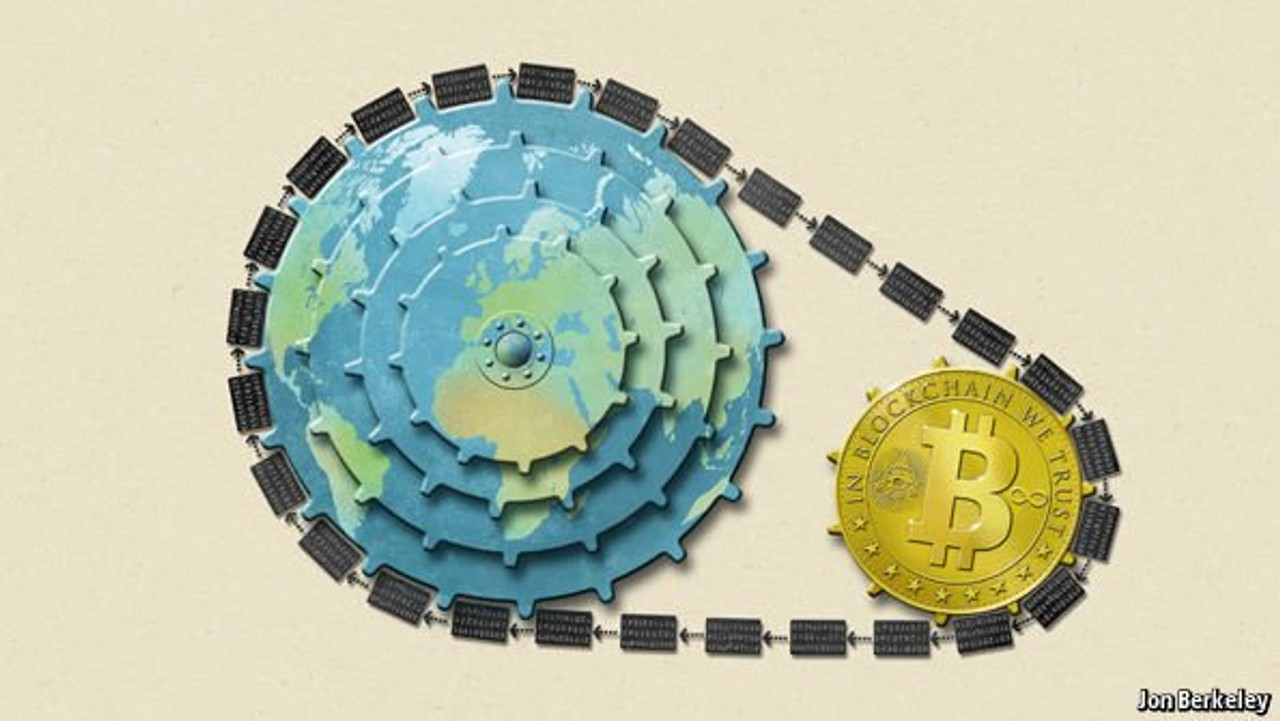
\includegraphics[width=\textwidth]{images/C0/20151031_LDD001_0.jpg}
%}
\setbeamertemplate{title page}[default][left]{\vspace*{0cm}}{\vspace*{0cm}}

% Definición variable bitcoin
\def\bitcoinC{\leavevmode\rlap{\hskip.5pt-}B}
\def\bitcoinA{%
  \leavevmode
  \vtop{\offinterlineskip %\bfseries
    \setbox0=\hbox{B}%
    \setbox2=\hbox to\wd0{\hfil\hskip-.03em
    \vrule height .3ex width .15ex\hskip .08em
    \vrule height .3ex width .15ex\hfil}
    \vbox{\copy2\box0}\box2}}
    
%---------------
\begin{document}

%###############
\section*{Título}
%###############

\begin{frame}[plain]

    \titlepage
    
    \note{
    \begin{itemize}
        \item Esta es la presentación asociada al documento de tesis "Activos digitales y estabilidad financiera" que presenté a fines de marzo de este año en UCEMA
        \item La propuesta es presentar un panorama general del documento con sus principales resultados y métodos asociados. En particular, la idea es identificar algunos aspectos vinculados a criptoactivos y estabilidad financiera en países emergentes. 
    \end{itemize}
    }
    
\end{frame}

%#####################
\section{C1. Introducción}
%#####################

\addtocounter{framenumber}{-1}
%--------------------------------
\subsection{Relevancia global}
%--------------------------------

\begin{frame}
\frametitle<1,2>{La \textcolor{blue}{prueba} de mercado aumentó...}


          
\end{frame}

\subsubsection{Capitalización}
%-----------------------------

\begin{frame}
\frametitle<1,2>{La \textcolor{blue}{capitalización} de mercado aumentó...}

        \begin{onlyenv}<1|handout:0>
        \begin{figure}[H]
        \begin{center}
         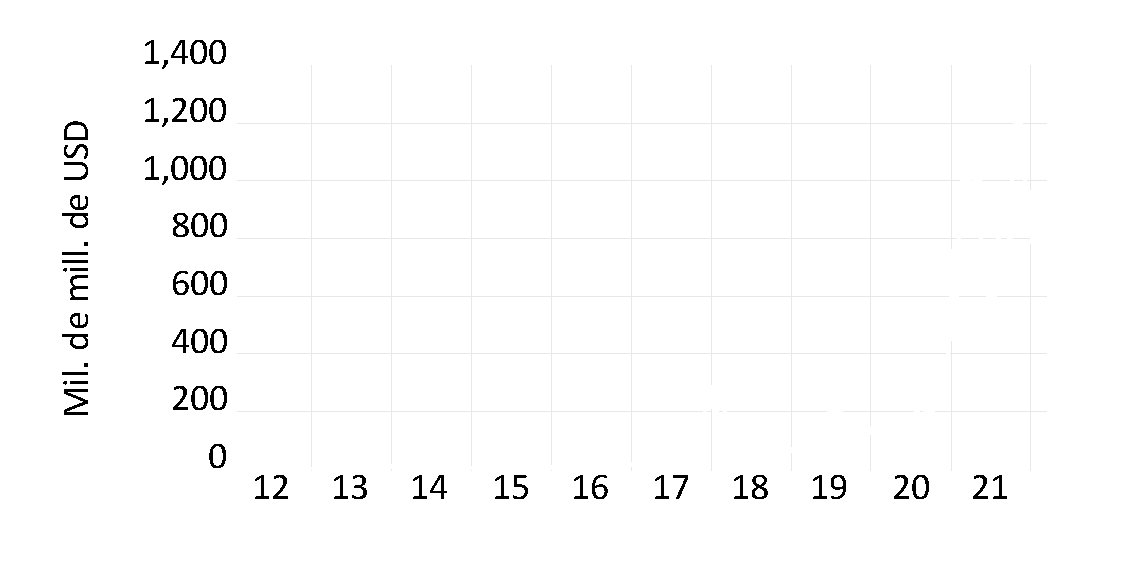
\includegraphics[width=1\textwidth]{images/C1/cap_axis.pdf}
         \end{center}
        \source{Fuente: \href{https://charts.coinmetrics.io/network-data/}{Coinmetrics}}
        \end{figure}
        \end{onlyenv}

        \begin{onlyenv}<2>
        \begin{figure}[H]
        \begin{center}
         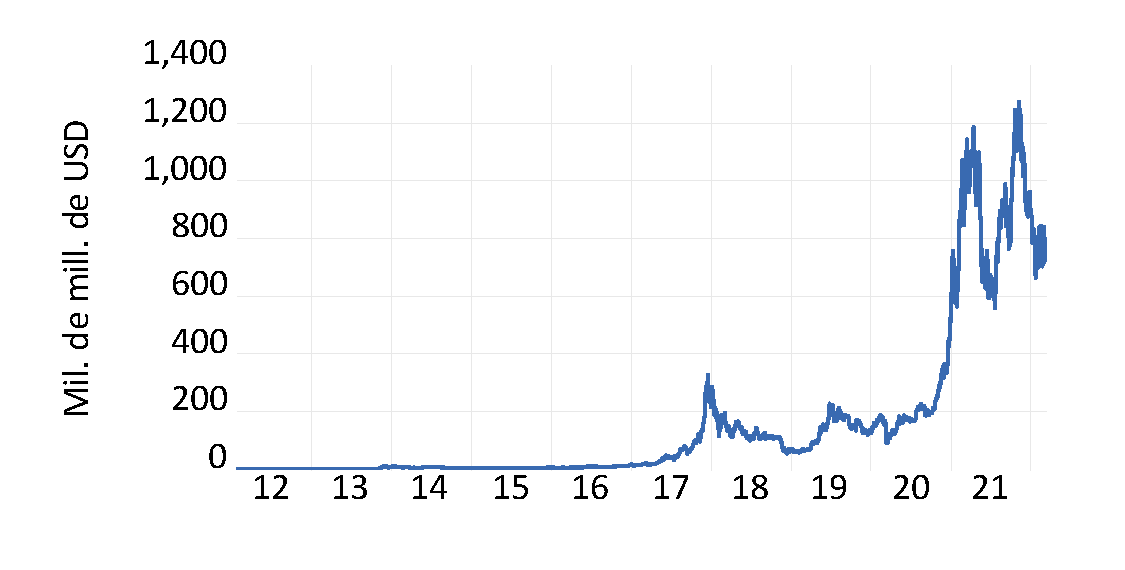
\includegraphics[width=1\textwidth]{images/C1/cap.pdf}
         \end{center}
        \source{Fuente: \href{https://charts.coinmetrics.io/network-data/}{Coinmetrics}}
        \end{figure}
        \end{onlyenv}
        
\note{
\begin{itemize}
    \item Una de las formas utilizadas habitualmente para evaluar la relevancia de bitcoin es observar la evolución en sus niveles de capitalización
    \item Valores máximos 2019: 200 mil millones de dólares aprox.
    \item Valor promedio últimos dos años: 800 mil millones de dólares aprox
    \item (900 mil millones con la suba de estos últimos días)
\end{itemize}
}
    
\end{frame}

\begin{frame}
\frametitle<1,2>{...en particular en los últimos dos años.}

        \begin{onlyenv}<1|handout:0>
        \begin{figure}[H]
        \begin{center}
         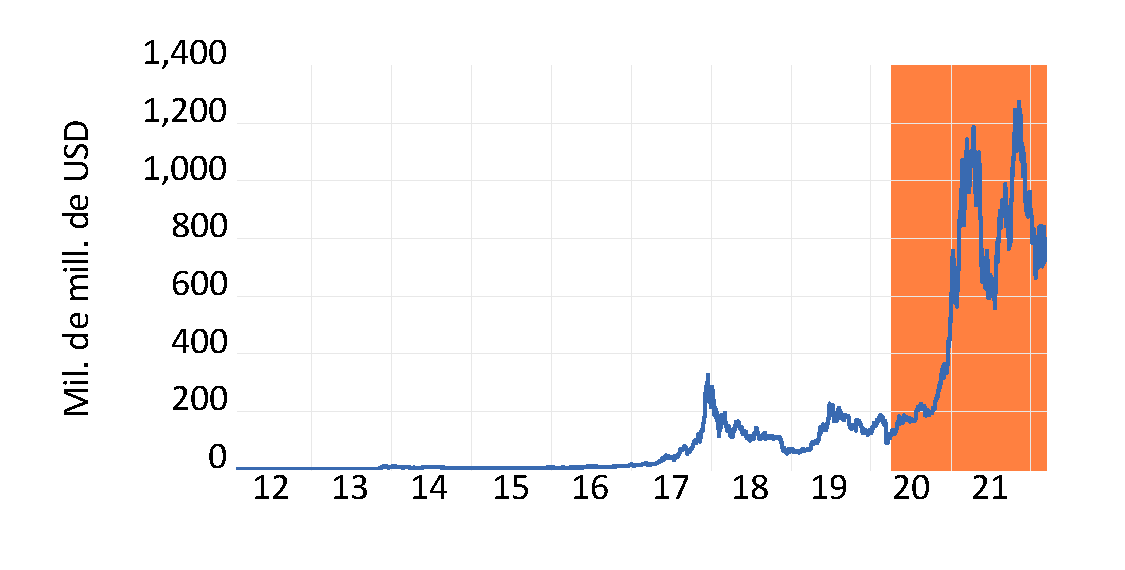
\includegraphics[width=1\textwidth]{images/C1/cap_shade.pdf}
         \end{center}
        \source{Fuente: \href{https://charts.coinmetrics.io/network-data/}{Coinmetrics}}
        \end{figure}
        \end{onlyenv}
        
        \begin{onlyenv}<2>
        \begin{figure}[H]
        \begin{center}
         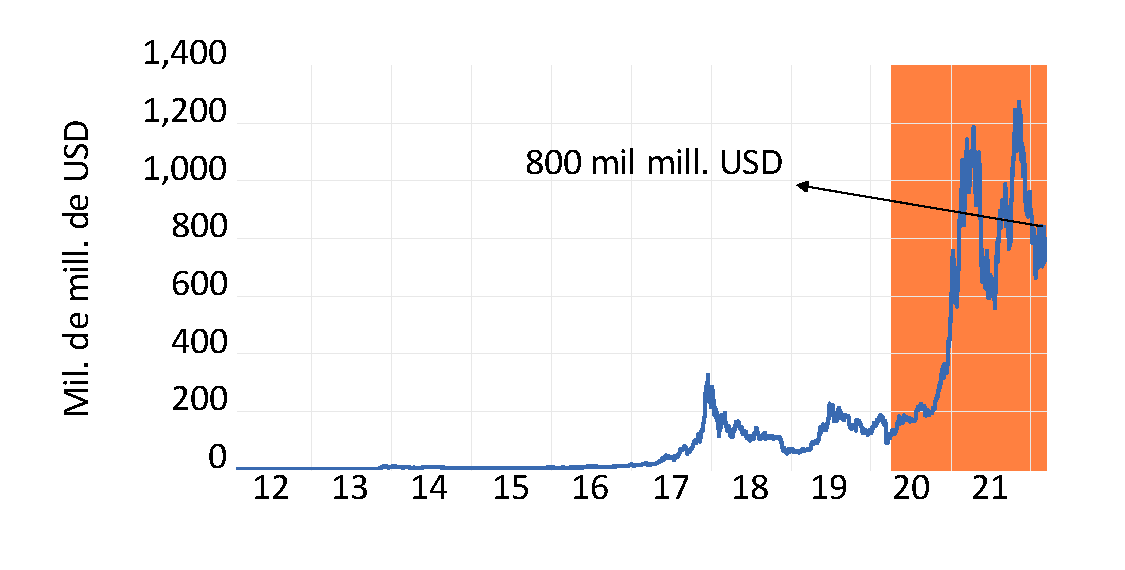
\includegraphics[width=1\textwidth]{images/C1/cap_shade_text.pdf}
         \end{center}
        \source{Fuente: \href{https://charts.coinmetrics.io/network-data/}{Coinmetrics}}
        \end{figure}
        \end{onlyenv}

\note{
\begin{itemize}
    \item 
\end{itemize}
}
    
\end{frame}

\subsubsection{Interconexiones}
%-----------------------------

\begin{frame}
\frametitle{Con relación a activos tradicionales...}

        \begin{figure}[H]
        \begin{center}
        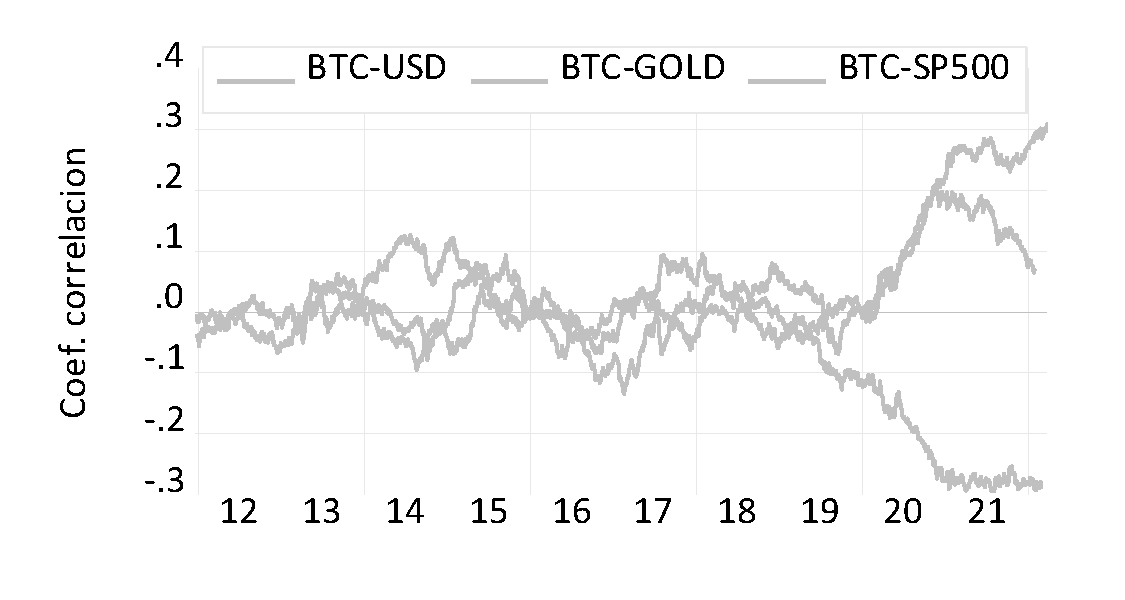
\includegraphics[width=1\textwidth]{images/C1/correlations/01.pdf}
        \end{center}
        \source{Fuente: \href{https://charts.coinmetrics.io/correlations/#435  }{Coinmetrics}}
        \end{figure}
        
\note{
\begin{itemize}
    \item Otra forma habitual de medir la relevancia de bitcoin (y ponderar sus riesgos) es buscar estimar su grado de vinculación con el sistema financiero tradicional.
    \item Por ejemplo, a través del análisis de asociación entre los rendimientos de bitcoin respecto al rendimiento de otros activos
    \item Cómo el SP500, el oro y el dólar. 
    \item \textcolor{gray}{Correlación de Spearman 360d}
    \item \textcolor{gray}{Fuente: Coinmentrics}
\end{itemize}
}
    
\end{frame}

\begin{frame}
\frametitle{... aumentó la correlación con el mercado de acciones...}

        \begin{figure}[H]
        \begin{center}
        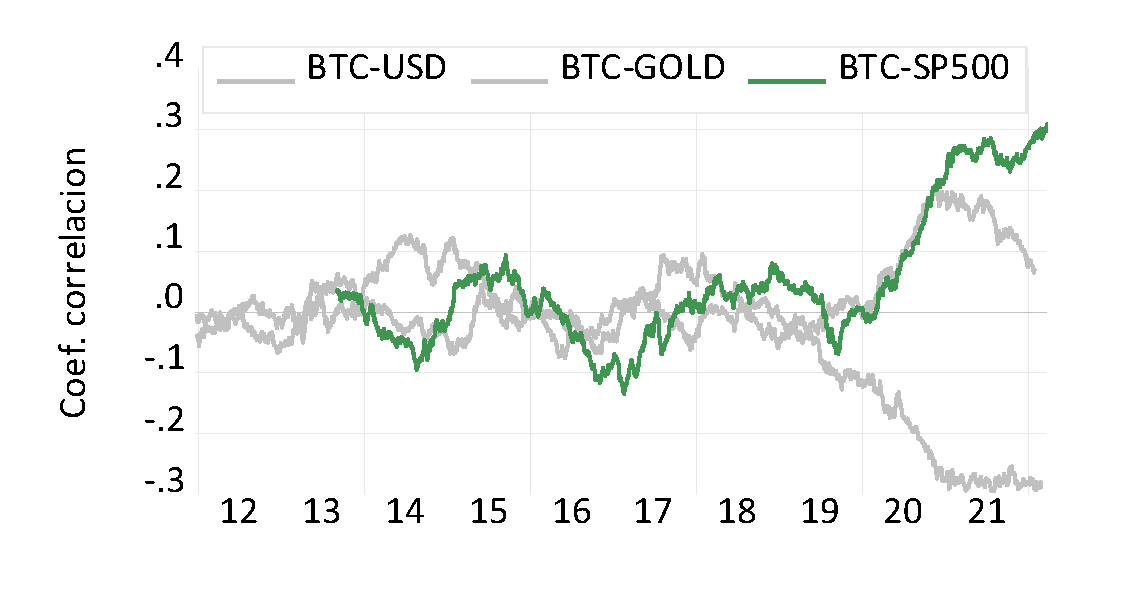
\includegraphics[width=1\textwidth]{images/C1/correlations/02.pdf}
         \end{center}
        \source{Fuente: \href{https://charts.coinmetrics.io/correlations/#3190}{Coinmetrics}} 
        \end{figure}

\note{
\begin{itemize}
    \item En los últimos dos años...
    \item ... se observa un incremento en el grado de asociación entre los rendimientos de bitcoin y el índice SP500...
    \item ... esto podría sugerir un mayor ingreso de inversores institucionales al mercado de bitcoin. 
\end{itemize}
}

\end{frame}

\begin{frame}
\frametitle{... disminuye la relación con el oro...}

        \begin{figure}[H]
        \begin{center}
        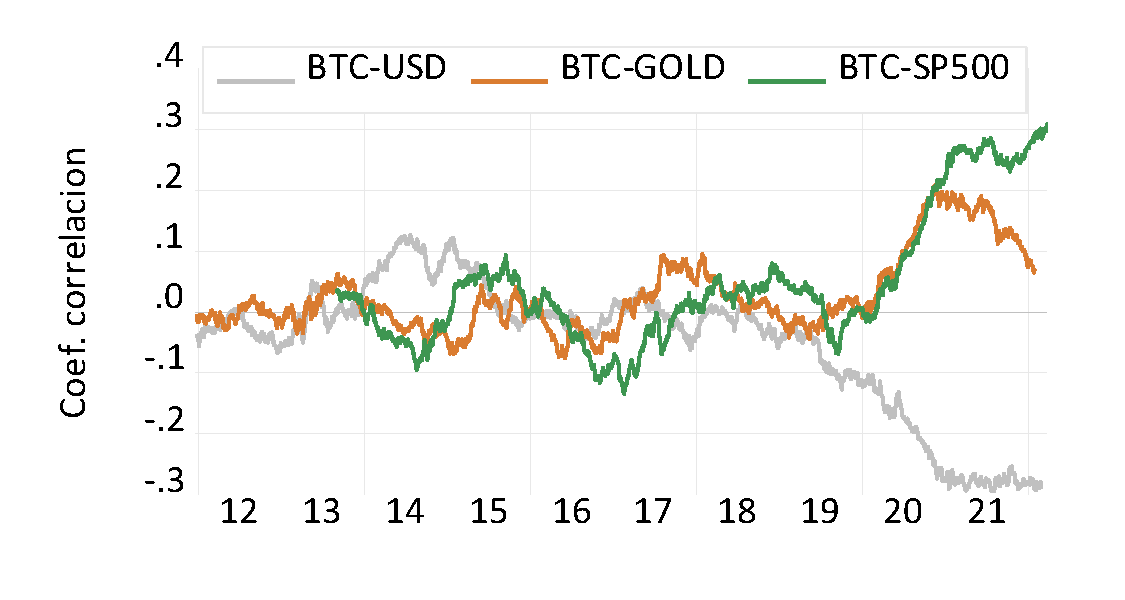
\includegraphics[width=1\textwidth]{images/C1/correlations/03.pdf}
         \end{center}
        \source{Fuente: \href{https://charts.coinmetrics.io/correlations/#3190}{Coinmetrics}} 
        \end{figure}

\note{
\begin{itemize}
    \item En el mismo período (últimos dos años)...
    \item Se observa un incremento inicial de la correlación con el oro pero luego esta correlación disminuye...
    \item ... esta situación pone en consideración las afirmaciones que sugieren que bitcoin puede situarse como un posible activo de resguardo.
\end{itemize}
}

\end{frame}

\begin{frame}
\frametitle{... y se consolida una relación negativa frente al dolar.}

        \begin{figure}[H]
        \begin{center}
        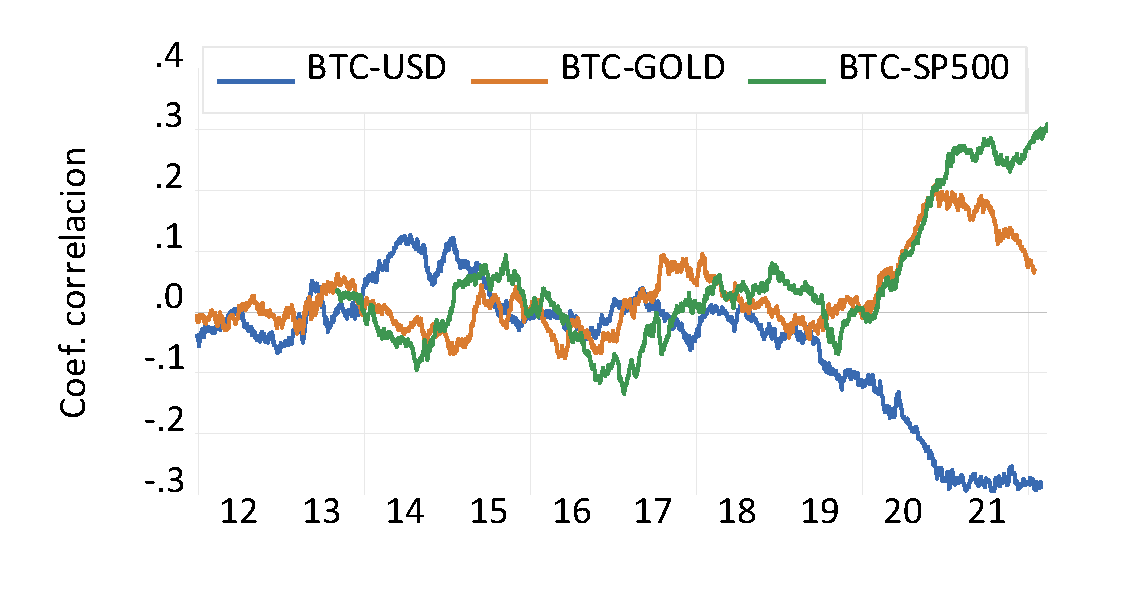
\includegraphics[width=1\textwidth]{images/C1/correlations/04.pdf}
         \end{center}
        \source{Fuente: \href{https://charts.coinmetrics.io/correlations/#3190}{Coinmetrics}} 
        \end{figure}

\note{
\begin{itemize}
    \item Finalmente, 
    \item También en el mismo período (últimos dos años)
    \item Se observa una disminución sostenida de la correlación con el índice dólar...
    \item ... esta situación podría sugerir que bitcoin puede situarse como un resguardo contra la inflación del dolar.
\end{itemize}
}

\end{frame}

\begin{frame}
\frametitle{Las entidades financieras con exposición a bitcoin se encuentra limitada}

        \begin{figure}[H]
        \begin{center}
        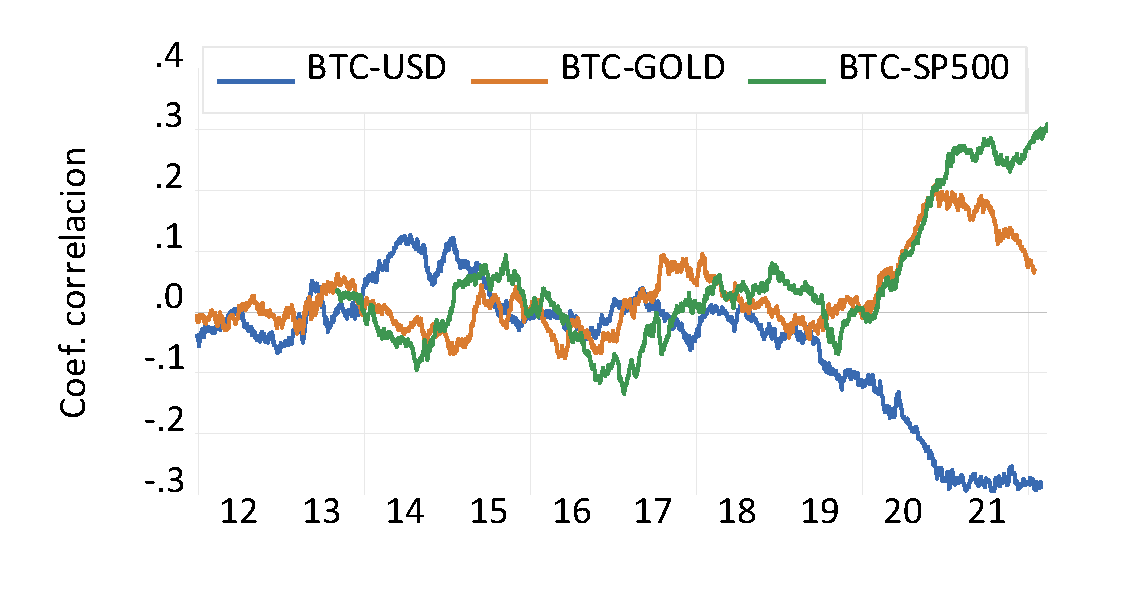
\includegraphics[width=1\textwidth]{images/C1/correlations/04.pdf}
         \end{center}
        \source{Fuente: \href{https://charts.coinmetrics.io/correlations/#3190}{Coinmetrics}} 
        \end{figure}

\note{
\begin{itemize}
    \item Finalmente, 
    \item También en el mismo período (últimos dos años)
    \item Se observa una disminución sostenida de la correlación con el índice dólar...
    \item ... esta situación podría sugerir que bitcoin puede situarse como un resguardo contra la inflación del dolar.
\end{itemize}
}

\end{frame}

\begin{frame}
\frametitle{Se incremento en la percepción de \textcolor{blue}{riesgo sistémico}..}

% slides 1/3 
\begin{columns}
    \begin{column}{0.5\textwidth}
        \begin{block}{FSB 2018}
        \begin{figure}[H]
        \begin{center}
         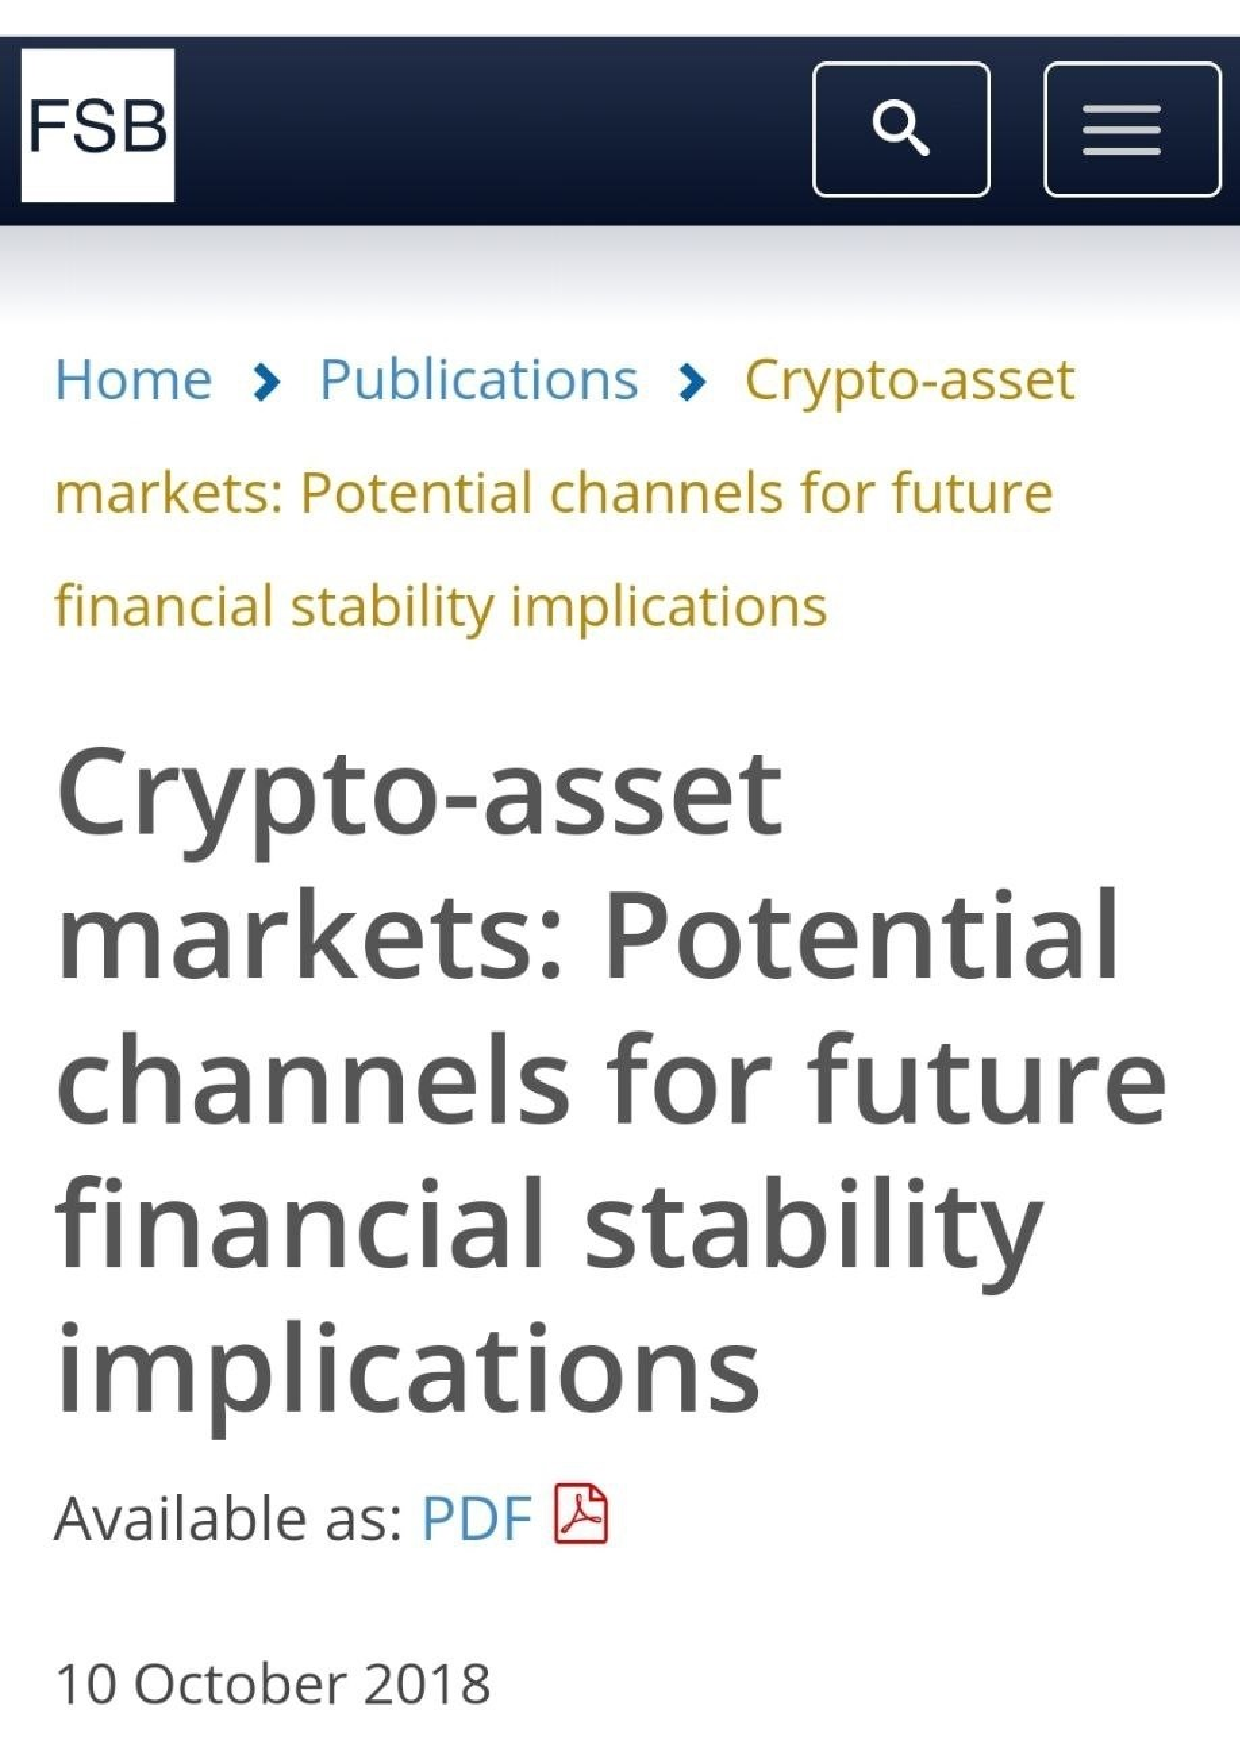
\includegraphics[width=0.6\textwidth]{images/C1/FSB 2018a.pdf}
         \end{center}
        \end{figure}
            \begin{figure}[H]
        \begin{center}
         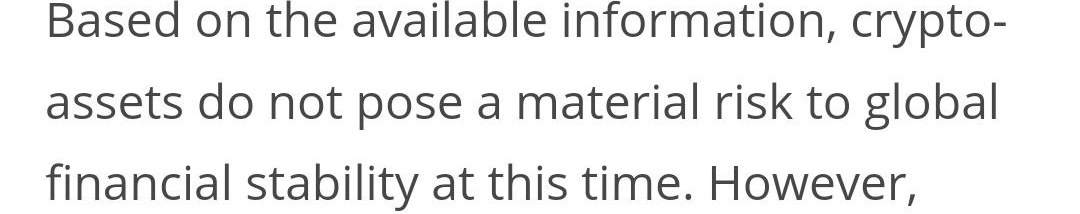
\includegraphics[width=0.8\textwidth]{images/C1/FSB 2018b}
         \end{center}
        \end{figure}
    \end{block}
    \end{column}
    \begin{column}{0.5\textwidth}  %%<--- here
        \begin{block}{FSB 2022}
        
        \begin{center}
         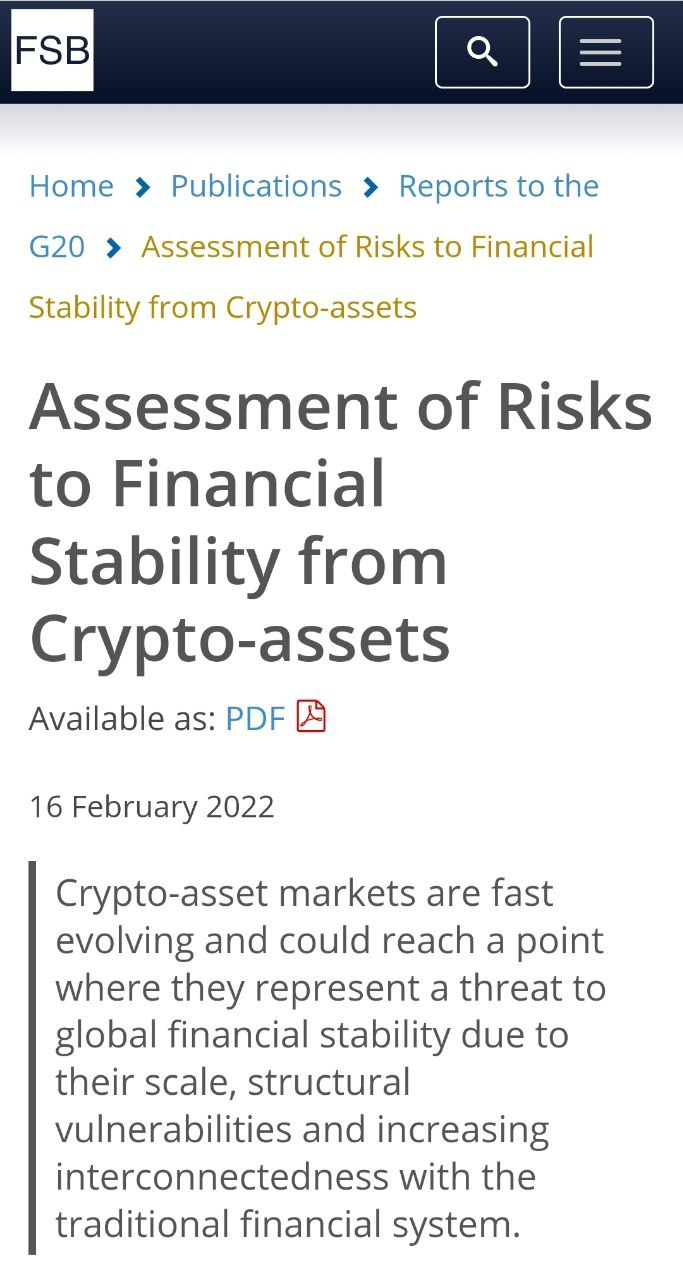
\includegraphics[width=0.6\textwidth]{images/C1/FSB 2022}
         \end{center}
             \end{block}
    \end{column}
\end{columns}

\note{
\begin{itemize}
    \item En este marco de mayor relevancia de bitcoin, se incrementa la percepción de los organismos de regulación y bancos centrales con relación a los riesgos asociados a bitcoin. 
    \item Para dar cuenta de esta posible mayor percepción del riesgo se pueden tener en cuenta, por ejemplo, las publicaciones del Consejo de Estabilidad Financiera (FSB).
\end{itemize}
}
\end{frame}
%----------

\addtocounter{framenumber}{-1}

% slides 3/3
\begin{frame}
\frametitle{...como sugieren las publicaciones del \textcolor{blue}{FSB}}

\begin{columns}
    \begin{column}{0.5\textwidth}
        \begin{block}{FSB 2018}
        
        \pgfsetfillopacity{0.4}% transparencia
    
         \begin{figure}[H]
        \begin{center}
         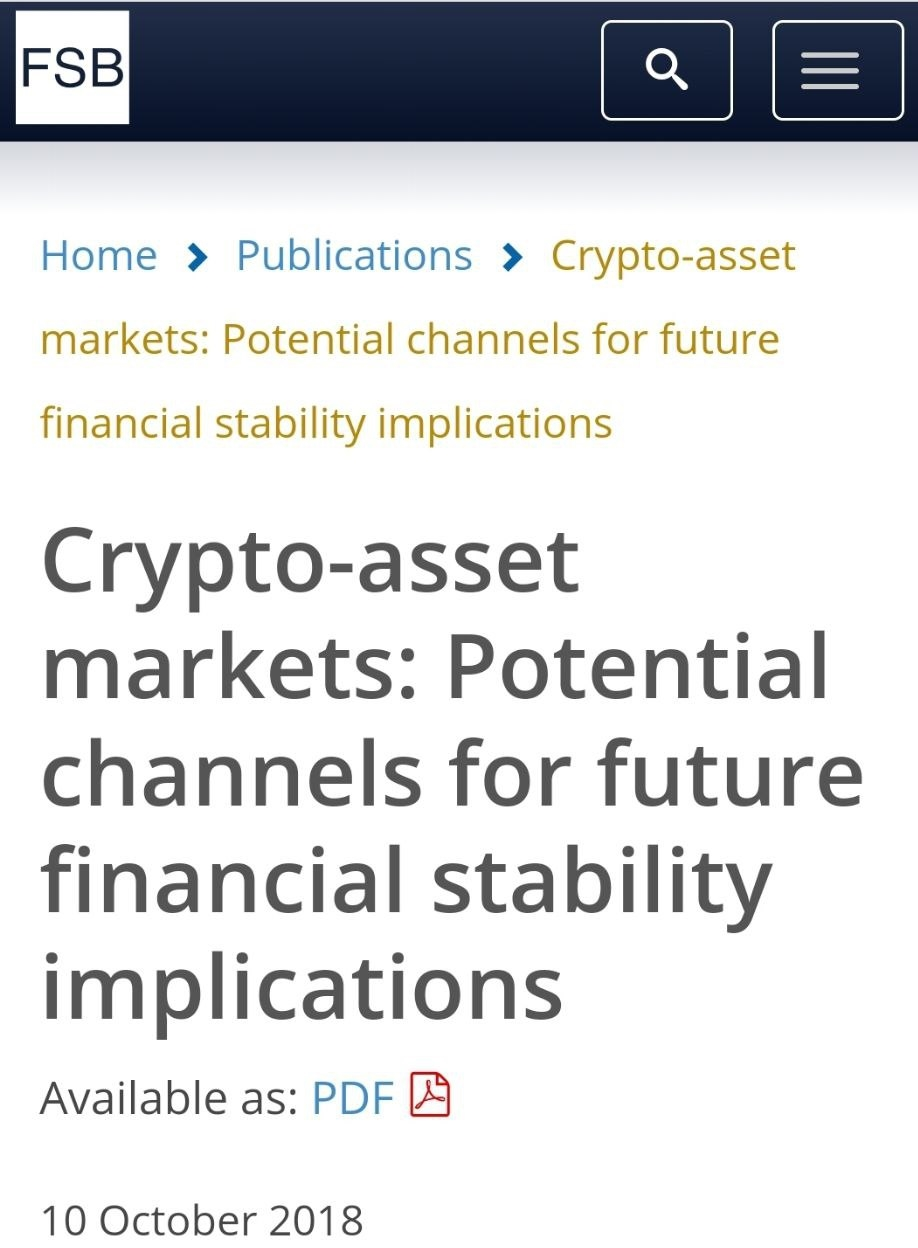
\includegraphics[width=0.6\textwidth]{images/C1/FSB 2018a}
         \end{center}
        \end{figure}
            \begin{figure}[H]
        \begin{center}
         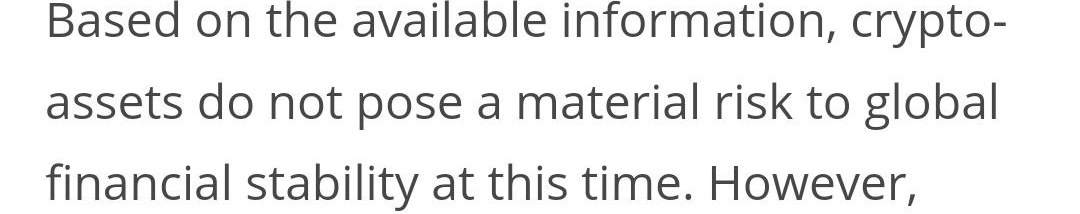
\includegraphics[width=0.8\textwidth]{images/C1/FSB 2018b}
         \end{center}
        \end{figure}
    \end{block}
    
    \pgfsetfillopacity{1}% transparencia
    
    % overlay 2018
        \begin{tikzpicture}[overlay][t] 
         \node[anchor=north east,xshift=5.5cm,yshift=2
         cm]{ 
\includegraphics[width=1\textwidth]{images/C1/FSB 2018b overlay.jpg}};
        \end{tikzpicture}
    
    \end{column}
    \begin{column}{0.5\textwidth}  %%<--- here
        \begin{block}{FSB 2022}
        
        \pgfsetfillopacity{0.4}% transparencia
        
        \begin{center}
         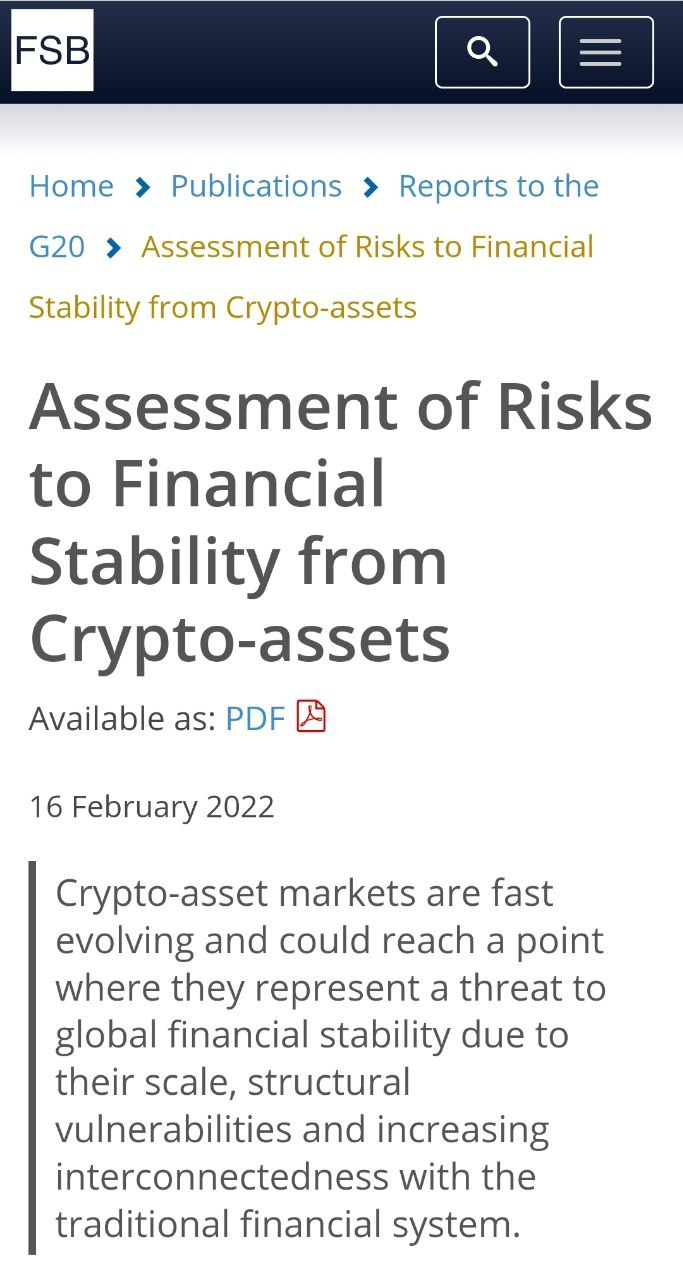
\includegraphics[width=0.6\textwidth]{images/C1/FSB 2022}
         \end{center}
             \end{block}
             
        \pgfsetfillopacity{1}% transparencia
             
        % overlay 2022
        \begin{tikzpicture}[overlay][t] 
         \node[anchor=north east,xshift=5.5cm,yshift=2.5
         cm]{ 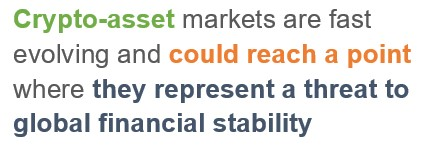
\includegraphics[width=0.9\textwidth]{images/C1/FSB 2022 overlay.jpg}};
        \end{tikzpicture}
             
    \end{column}
    
\end{columns}

\note{
\begin{itemize}
    \item Si se comprara, por ejemplo, la primera publicación del FSB respecto a la última (de febrero de este año), se encuentran conclusiones diferentes:
    \item 2018: "Basado en la información disponible, \textbf{los criptoactivos no suponen en ese momento un riesgo para la estabilidad financiera global}"
    \item 2022: "Los mercados de criptoactivos están evolucionando rápidamente y \textbf{podrían llegar a representar una amenaza para la estabilidad financiera mundial"}
\end{itemize}
}
\end{frame}
%----------

% IMF y BOE

\begin{frame}
\frametitle{... y las publicaciones del \textcolor{blue}{IMF} y el \textcolor{blue}{BoE} ...}

% slides 1/3 
\begin{columns}
    \begin{column}{0.5\textwidth}
        \begin{block}{BoE 2021}
        \begin{figure}[H]
        \begin{center}
         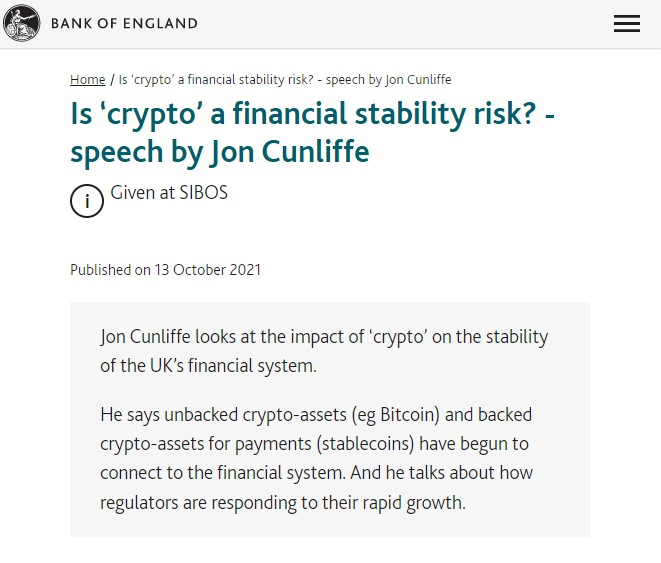
\includegraphics[width=1\textwidth]{images/C1/global/BoE 2021.jpg}
         \end{center}
        \end{figure}
              \end{block}
    \end{column}
    \begin{column}{0.5\textwidth}  %%<--- here
        \begin{block}{IMF 2021}
        \begin{center}
         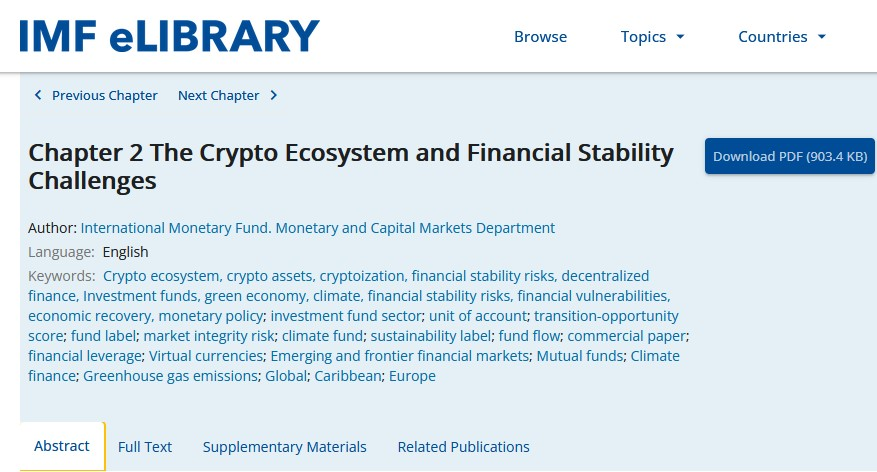
\includegraphics[width=1\textwidth]{images/C1/global/IMF 2021d.jpg}
         \end{center}
             \end{block}
    \end{column}
\end{columns}

\note{
\begin{itemize}
\item En el mismo sentido se encuentran las últimas publicaciones del BoE y del IMF (a través de su GFSR)
\end{itemize}
}
\end{frame}
%----------

%-------------------------------
\subsection{Relevancia local}
%-------------------------------

\subsubsection{Oferta}
%------------------

\begin{frame}
\frametitle<1,2>{A nivel \textcolor{blue}{local} se expande la \textcolor{dgreen}{oferta}...}

    \begin{figure}
    \centering
        \includegraphics<1>[width=1\textwidth]{images/C1/arg/bloomberg (1).jpg}
        \includegraphics<2|handout:0>[width=1\textwidth]{images/C1/arg/afa.jpg}
        \vspace{-5mm}
        \caption*{Fuente: \href{https://www.bloomberg.com/news/articles/2022-03-09/cryptocurrencies-prove-a-lifeline-in-argentina-s-chaotic-economy}{Bloomberg}}
    \end{figure}
    
    \note{
    \begin{itemize}
        \item A nivel local, 
        \item Se observa una creciente oferta de proveedores de bitcoin
        \item Como reflejan estas publicidades de operadores locales en la vía pública
        \item Fuente: Bloomberg
        \item nota vinculada a la reciente regulación del BCRA https://www.ft.com/content/4dae4742-c339-4414-9bfa-4739df6e5248
    \end{itemize}
    }
    
\end{frame}
%----------

\subsubsection{Demanda}
%------------------

\begin{frame}
\frametitle{A la vez que se incrementa la \textcolor{dgreen}{demanda}...}
    \begin{figure}
    \centering
        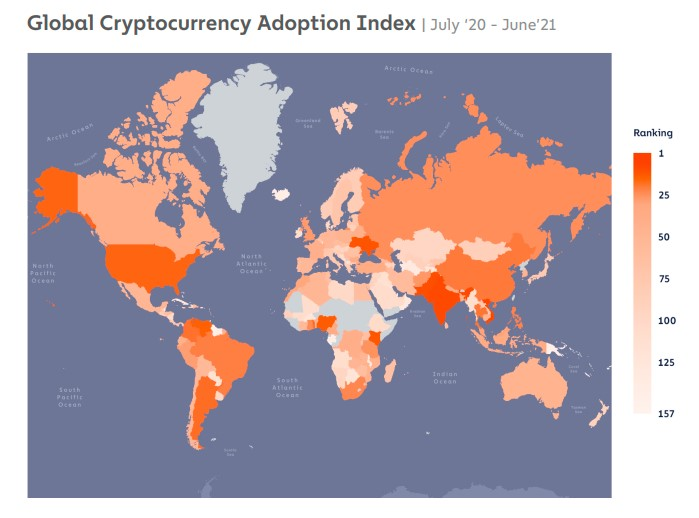
\includegraphics[width=0.8\textwidth]{images/C1/arg/arg_demanda (1).jpg}
        \caption*{Fuente: \href{https://blog.chainalysis.com/reports/2021-global-crypto-adoption-index/}{Chainalysis}}
        \end{figure}
        
    \note{
    \begin{itemize}
        \item Al mismo tiempo que se incrementa la oferta se puede identificar un incremento en la demanda.
        \item Se puede dar cuenta de este incremento en la demanda por, por ejemplo, a través del índice de adopción global de la empresa Chainalysis ...
        \item ... de octubre 2021 ...
        \item ... donde Argentina figura en el número 10° (primer país en AL, Brasil 14°).
    \end{itemize}
    }

\end{frame}

\begin{frame}
\frametitle{... en particular \textcolor{blue}{p2p}}.

    \begin{figure}
    \centering
        \includegraphics<1>[width=0.8\textwidth]{images/C1/global/IMF 2021b.jpg}
        \includegraphics<2>[width=0.8\textwidth]{images/C1/global/IMF 2021b - copia.jpg}
        \vspace{-5mm}
        \caption*{Fuente: \href{https://www.imf.org/-/media/Files/Publications/GFSR/2021/October/English/ch2.ashx}{IMF (2021) GFSR}}
        \end{figure}
        
    \note{
    \begin{itemize}
        \item Este incremento en la demanda se observa con particular énfasis en las operaciones directas entre personas (p2p)
        \item Estos datos son tomados del GFSR del IMF de octubre de 2021. 
        \item ... donde Argentina 5° Binance. 
    \end{itemize}
    }

\end{frame}

\begin{frame}
\frametitle{... en particular \textcolor{blue}{p2p}}.

    \begin{figure}
    \centering
        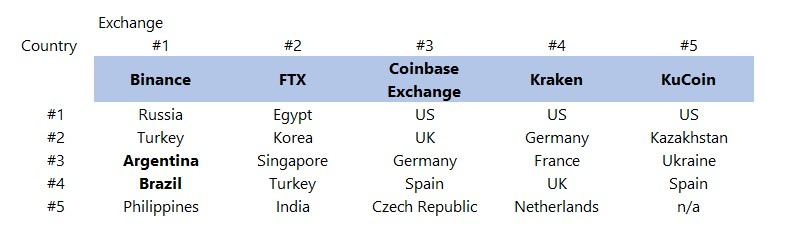
\includegraphics[
        [width=0,scale=0.55]{images/C1/global/p2p.jpg}
        \vspace{5mm}
        \caption*{Fuente: \href{https://www.similarweb.com/es/}{Similarweb}}
        \end{figure}
        
    \note{
    \begin{itemize}
        \item 
    \end{itemize}
    }

\end{frame}

\begin{frame}
\frametitle{Ranking de precios de compra y venta local}.

    \begin{figure}
    \centering
        \includegraphics<1>[width=1\textwidth]{images/C1/arg/coinmonitor.jpg}
        \caption*{Fuente: \href{https://www.coinmonitor.info/}{CoinMonitor Argentina}}
        \end{figure}
        
    \note{
    \begin{itemize}
        \item La oferta y demanda de bitcon local se puede sintetizar en el cuadro con el RANKING DE LOS MEJORES PRECIOS FINALES -comisiones incluídas- DE LOS PRINCIPALES BROKERS O EXCHANGES DE INTERES EN ARGENTINA 
        \item de la página local "CoinMonitor"
        \item aproximadamente 15 operadores
    \end{itemize}
    }

\end{frame}

%----------------------------------
\subsection{Taxonomía/clasificación}
%-----------------------------------

\begin{frame}
\frametitle{De manera preliminar, la taxonomía de criptoactivos es la siguiente}.

    \begin{figure}
    \centering
        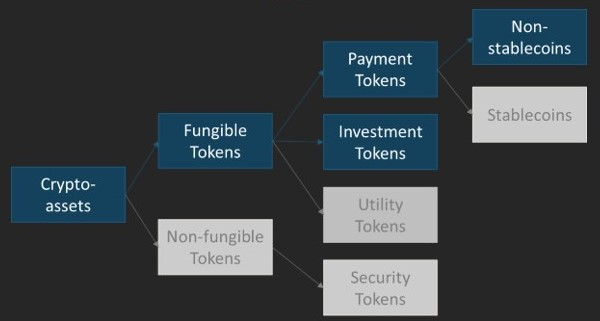
\includegraphics[width=1\textwidth]{images/C1/classification/classification.jpg}
        \caption*{Fuente: elaboración propia en base a IMF}
        \end{figure}
        
    \note{
    \begin{itemize}
        \item 
    \end{itemize}
    }

\end{frame}

%---------------------
\subsection{Preguntas}
%---------------------

\begin{frame}

\Large
\centering
¿Un incremento en la demanda de bitcoin en Argentina puede afectar la estabilidad financiera?

    \note{
    \begin{itemize}
        \item En ese marco de aumento de la relevancia de bitcoin en particular en los últimos dos años...
        \item ... se plantea la pregunta general de la investigación:
        \item ¿Un incremento en la demanda de bitcoin ...?
    \end{itemize}
    }
    
\end{frame}
%----------

\begin{frame}

\begin{itemize}
    \item[] \onslide<1>{\textcolor{blue}{\textbf{Oferta}}}
    \item[] \onslide<2>{¿Es posible que \textcolor{blue}{bitcoin} puede funcionar como una \textcolor{blue}{tecnología equivalente al dinero}?}
    
    \vspace{5mm}
    \item[] \onslide<1>{\textcolor{dgreen}{\textbf{Demanda}}}
    \item[] \onslide<3>{¿Es posible que la \textcolor{dgreen}{demanda de bitcoin} se encuentre asociada a las opiniones de un grupo de \textcolor{dgreen}{actores influyentes}?}
    
    \vspace{5mm}
    \item[] \onslide<1>{\textcolor{orange}{\textbf{Implicancias}}}
    \item[] \onslide<4>{¿Un \textcolor{orange}{mayor} nivel de \textcolor{orange}{adopción} de bitcoin puede generar incrementos en la \textcolor{orange}{volatilidad del tipo de cambio} entre pesos y dólares en Argentina?}
\end{itemize}

    \note{
    \begin{itemize}
        \item Para responder a esa pregunta general, se proponen \textbf{tres preguntas específicas}. 
        \item Las dos primeras se vinculan al análisis del mercado de oferta y demanda de bitcoin.
        \item La última se asocia a las implicancias de un mayor grado de adopción de bitcoin en Argentina. 
        \item Las preguntas específicas son: ..., ..., ...
    \end{itemize}
    }
    
\end{frame}

%---------------------
\subsection{Overviews}
%---------------------

%-----------------------------------------------------
\subsubsection{Perspectiva general de la investigación}
%-----------------------------------------------------

\begin{frame}
\frametitle{Perspectiva general}
%------------------------------
\begin{columns}

    \begin{column}{0.50\textwidth}
    \vspace{-5pt}
    \begin{block}{\textcolor{blue}{Oferta}}
        \begin{column}{0.1\textwidth}
        \vspace{-10pt} % estos espacios negativos son claves para alinear
            \tiny
            \begin{align*}
            c_{1,t}+\Phi_t \le y\\
            c_{2,t+1}\le\Phi_{t+1}^R\\
            N_{t-1}\textcolor{red}{x_t} \cdot \Phi_{t-1}^{\textbf{DLT}}=N_t(*)
            \end{align*}
        \end{column}
        \begin{column}{0.35\textwidth}  
            \begin{figure}[H]
            \begin{center}
             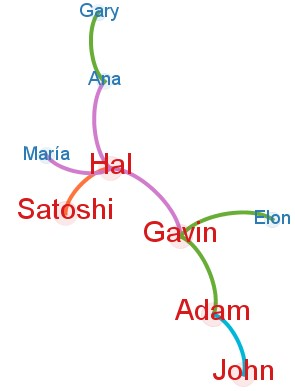
\includegraphics[width=1\textwidth]{images/C2/c2_simul_red5.jpg}
             \end{center}
            \end{figure}
            \end{column}
    \end{block}
    \begin{block}{\textcolor{dgreen}{Demanda}}
        \vspace{-10pt}
            \tiny
              \begin{align*}
              v_{t}^{\$}{M_{t}^{\$}}&={N_{t}^{\$}\left(*\right)}+(1-\lambda_t){N_{t}^{\$}\left(*\right)}\\
              v_{t}^{\bitcoinA}{M_{t}^{\bitcoinA}}&={N_{t}^{\bitcoinA}\left(*\right)+\lambda_tN_{t}^{\$}\left(*\right)}\\
              \lambda_t&=\textcolor{blue!70}{S}(\textcolor{red}{\mu_t})
            \end{align*}
    \vspace{-20pt}
            \begin{figure}[t!]
            \begin{center}
            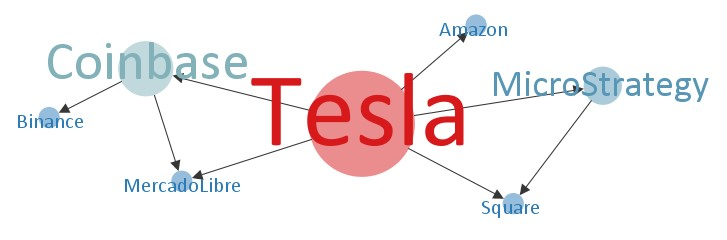
\includegraphics[width=0.6\textwidth]{images/C3/c3_simul_influ3.jpg}
             \end{center}
            \end{figure}
            
    \end{block}
    \end{column}
    
    \begin{column}{0.55\textwidth}
    
    \begin{block}{\textcolor{orange}{Implicancias}}
    \tiny

    \begin{align*}
    v^{\$a}_1 M^{\$a}_1&=P_1^{{\$a}} + \lambda_1 (1-\alpha_1) R_1^{{\$a}} + (1-\lambda_1) \textcolor{blue!60}{\rho_1}  R_1^{{\$a}}\\
    v_1^{\$} M_1^{\$}&=(1-\lambda_1) \textcolor{green!70}{\delta_1} R_1^{\$a}\\
    v_1^{\bitcoinA} M_1^{\bitcoinA}&=\textcolor{orange}{\lambda_1}  \alpha_1 R_1^{\$a} + (1-\lambda_1) \textcolor{red}{\beta_1} R_1^{\$a}\\
    e_t^{{\$a};{\$}}&=\frac{v_1^{\$a}}{v_1^{\$}}
    \end{align*}
    
    \vspace{-5pt}
    
    \begin{figure}[H]
    \begin{center}
     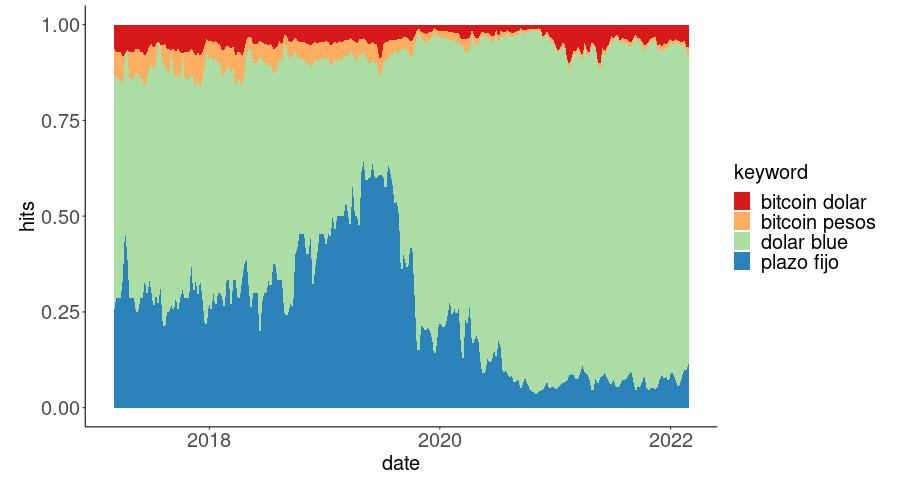
\includegraphics[width=1\textwidth]{images/C4/Rplot001.png}
     \end{center}
    \end{figure}
    
    \end{block}

    \end{column}
\end{columns}

\note{
\begin{itemize}
    \item Para poder dar respuestas a cada una de dichas preguntas se propone una evaluación conceptual y una evaluación empírica. 
    \item Evaluación conceptual
        \begin{itemize}
        \item Modelos OLG para los tres objetivos, con el mismo entorno (previsión perfecta, estacionariedad, un solo bien, dos generaciones que viven dos períodos, tiempo infinito).
        \end{itemize}
    \item Evaluación empírica
        \begin{itemize}
        \item Objetivo 1 y 2: técnicas de análisis de red
        \item Objetivo 3: datos de Google Trend (no hay posibilidad de georeferenciar datos de la blockchain o Twitter).
        \end{itemize}
\end{itemize}
}

\end{frame}
%----------




%###############
\section{C2. Oferta}
%###############

\addtocounter{framenumber}{-1}

\begin{frame}
\frametitle{Perspectiva general}
%------------------------------
\begin{columns}

    \begin{column}{0.50\textwidth}
    \vspace{-5pt}
    \begin{block}{\textcolor{blue}{Oferta}}
        \begin{column}{0.1\textwidth}
        \vspace{-10pt} % estos espacios negativos son claves para alinear
            \tiny
            \begin{align*}
            c_{1,t}+\Phi_t \le y\\
            c_{2,t+1}\le\Phi_{t+1}^R\\
            N_{t-1}\textcolor{red}{x_t} \cdot \Phi_{t-1}^{\textbf{DLT}}=N_t(*)
            \end{align*}
        \end{column}
        \begin{column}{0.35\textwidth}  
            \begin{figure}[H]
            \begin{center}
             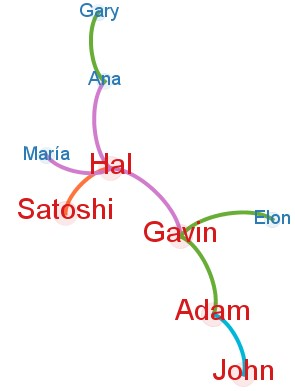
\includegraphics[width=1\textwidth]{images/C2/c2_simul_red5.jpg}
             \end{center}
            \end{figure}
            \end{column}
    \end{block}
    
    \pgfsetfillopacity{0.2}
    
    \begin{block}{Demanda}
        \vspace{-10pt}
            \tiny
              \begin{align*}
              v_{t}^{\$}{M_{t}^{\$}}&={N_{t}^{\$}\left(*\right)}+(1-\lambda_t){N_{t}^{\$}\left(*\right)}\\
              v_{t}^{\bitcoinA}{M_{t}^{\bitcoinA}}&={N_{t}^{\bitcoinA}\left(*\right)+\lambda_tN_{t}^{\$}\left(*\right)}\\
              \lambda_t&=\textcolor{blue!70}{S}(\textcolor{red}{\mu_t})
            \end{align*}
    \vspace{-20pt}
            \begin{figure}[t!]
            \begin{center}
            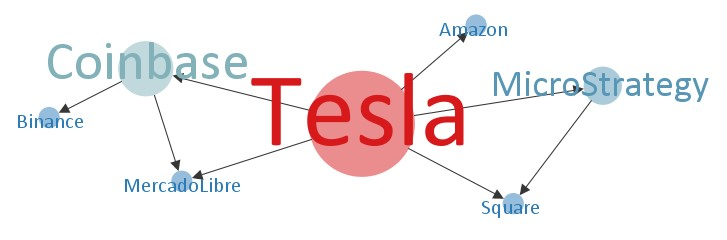
\includegraphics[width=0.6\textwidth]{images/C3/c3_simul_influ3.jpg}
             \end{center}
            \end{figure}
            
    \end{block}
    \end{column}
    
    \begin{column}{0.55\textwidth}
    
    \begin{block}{Implicancias}
    \tiny

    \begin{align*}
    v^{\$a}_1 M^{\$a}_1&=P_1^{{\$a}} + \lambda_1 (1-\alpha_1) R_1^{{\$a}} + (1-\lambda_1) \textcolor{blue!60}{\rho_1}  R_1^{{\$a}}\\
    v_1^{\$} M_1^{\$}&=(1-\lambda_1) \textcolor{green!70}{\delta_1} R_1^{\$a}\\
    v_1^{\bitcoinA} M_1^{\bitcoinA}&=\textcolor{orange}{\lambda_1}  \alpha_1 R_1^{\$a} + (1-\lambda_1) \textcolor{red}{\beta_1} R_1^{\$a}\\
    e_t^{{\$a};{\$}}&=\frac{v_1^{\$a}}{v_1^{\$}}
    \end{align*}
    
    \vspace{-5pt}
    
    \begin{figure}[H]
    \begin{center}
     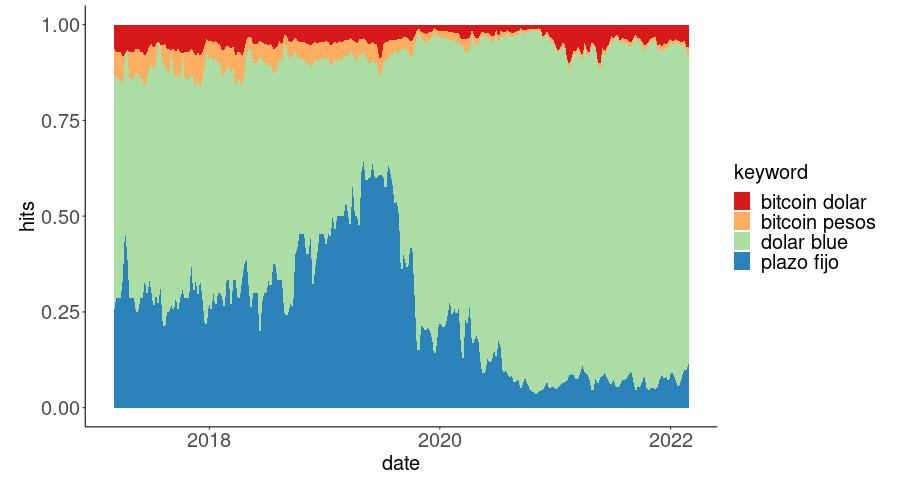
\includegraphics[width=1\textwidth]{images/C4/Rplot001.png}
     \end{center}
    \end{figure}
    
    \pgfsetfillopacity{1}
    
    \end{block}

    \end{column}
\end{columns}

\note{
\begin{itemize}
    \item Entonces, a partir de este panorama general de las diferentes partes y métodos de evaluación de la investigación, 
    \item Se comienza el análisis de la primera parte, 
    \item la cual se encuentra asociada a las características de oferta de bitcoin. 
\end{itemize}
}

\end{frame}
%----------

\subsection{Objetivos}
\begin{frame}{}

    \textcolor{blue}{\textbf{Objetivo}}.\\
    \vspace{5mm}
    \begin{itemize}
        \setlength\itemsep{1em}
        
        \item[] Describir las \textcolor{blue}{características de oferta} del sistema bitcoin.\\ 
        
        \item[] Analizar a partir de un \textcolor{blue}{modelo} si la tecnología de red distribuida puede funcionar como una tecnología equivalente al dinero.\\
        \item[] Evaluar empíricamente el modelo a partir de los \textcolor{blue}{datos de la cadena de bloques} de bitcoin.
    \end{itemize}
 
    \vspace{5mm}
    \textcolor{dgreen}{\textbf{Conjetura}}. 
    \vspace{5mm}
    \begin{itemize}
    \item[] La tecnología de red distribuida DLT que subyace al sistema bitcoin puede funcionar como una \textcolor{dgreen}{tecnología funcionalmente equivalente al dinero}.
    \end{itemize}


\note{
\begin{itemize}
    \item Para esta primera parte de la investigación, se plantean tres objetivos específicos
    \item (Leer cada objetivo)
    \item A su vez, se plantea la siguiente conjetura:
    \item (Leer la conjetura)
\end{itemize}
}
    
\end{frame}
%----------

\subsection{Definiciones}
%------------------------
\begin{frame}

\vspace{5mm}
\begin{displayquote}
El \textcolor{blue}{dinero} es equivalente a una forma primitiva de \textcolor{dgreen}{memoria}. 
\end{displayquote}
\raggedleft \cite{Kocherlakota1998} \\ \citetitle{Kocherlakota1998}

\vspace{5mm}
\begin{block}<2>{DLT como memoria}
La \textcolor{red}{DLT} es un registro público equivalente a un proceso de \textcolor{dgreen}{memoria} social. El dinero es equivalente a una forma primitiva de memoria social. Por lo tanto, una DLT sería un proceso tecnológico equivalente al \textcolor{blue}{dinero}.
\end{block}

\note{
\begin{itemize}
    \item Para esta primera parte de la investigación se propone retomar algunas \textbf{definiciones clásicas de dinero} como, por ejemplo, la idea de dinero como proceso de memoria social (a diferencia de la definición funcional clásica de dinero como medio de pago, reserva de valor o unidad de cuenta).
    \item En este sentido, \textbf{Kocherlakota} indica en "Money is Memory" que (leer cita)
    \item A partir de esa definición, se propone el siguiente concepto asociado a la DLT: (leer el recurado sobre DLT)
    \item En este marco, Shin (jefe de investigaciones en el BIS) indica que "la idea de dinero como tecnología de memoria aplicada en un registro universal era una propuesta teórica no observable". Pero que "los avances asociados a las DLT han hecho posible la existencia concreta de tal registro". Por lo tanto: "los activos digitales pueden ser considerados una tecnología equivalente al dinero"
    \href{http://www.overleaf.com}{Distributed ledgers and  the governance of money}
\end{itemize}
}
    
\end{frame}
%----------

\begin{frame}

\vspace{5mm}
\begin{displayquote}
El \textcolor{blue}{dinero} en la economía moderna es una forma especial de pagaré o, en términos económicos, un activo financiero. El dinero es un tipo especial de pagaré en el que todos tienen \textcolor{dgreen}{confianza}. 
\end{displayquote}
\raggedleft \cite{Mcleay2014c} \\ \citetitle{Mcleay2014c}

\vspace{5mm}
\begin{block}<2>{POW-confianza}
La DLT de bitcoin basa la \textcolor{dgreen}{confianza} en su sistema de registro en un mecanismo de consenso específico denominado \textcolor{red}{POW}.  \parencite{Ali2014}.
\end{block}

\note{
\begin{itemize}
    \item Una segunda definición de dinero relevante para esta primera parte de la investigación es la que asocia dinero a un proceso de confianza. 
    \item En este sentido, el Banco de Inglaterra, en una publicación muy influyente sobre la naturaleza del dinero de 2014 indica que (leer cita).
    \item A partir de este concepto, se propone un segundo concepto asociad a la DLT: (leer recuadro)
\end{itemize}
}
    
\end{frame}
%----------



\subsection{Evaluación conceptual y empírica}
%--------------------------------------------

% overview
\begin{frame}{Evaluación conceptual y empírica}
    
    \begin{block}{Modelo}
    \begin{minipage}[t][.20\textheight][t]{\textwidth}
        \begin{column}{0.30\textwidth}
        \vspace{-10pt} % estos espacios negativos son claves para alinear
            \tiny
            \begin{align*}
            {c_{1,t}+\Phi_t \le y}\\
            c_{2,t+1}\le \Phi_{t+1}^R\\
            {N_{t-1}\textcolor{red}{x_t} \cdot \Phi_{t-1}^{\textbf{DLT}}=N_t(y-c_{1,t})}
            \end{align*}
        \end{column}
        \begin{column}{0.45\textwidth}
        \end{column}
    \end{minipage}
    \end{block}

    \begin{block}{Evaluación empírica}
    
    \begin{minipage}[t][.40\textheight][t]{\textwidth}

    \begin{columns}
    \begin{column}{0.3\textwidth}
    \tiny
    \begin{figure}[H]
        \begin{center}
             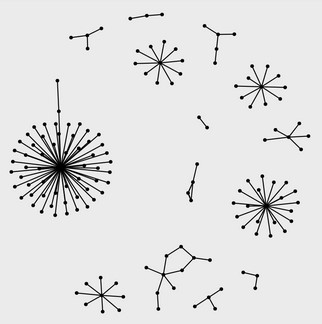
\includegraphics[width=0.8\textwidth]{images/C2/2009/sinfiltro.jpg}
         \end{center}
    \end{figure}
    \end{column}
    \begin{column}{0.3\textwidth}  
    \tiny
    \begin{figure}[H]
        \begin{center}
         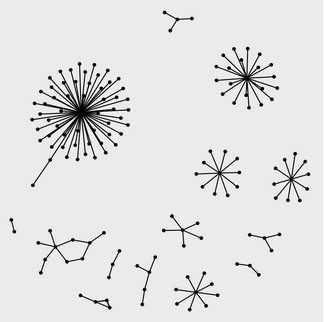
\includegraphics[width=0.75\textwidth]{images/C2/2009/filtradaa.jpg}
         \end{center}
    \end{figure}
    \end{column}
    \begin{column}{0.3\textwidth}  
    \tiny
    \begin{figure}[H]
        \begin{center}
         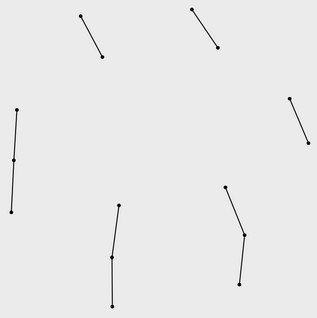
\includegraphics[width=0.8\textwidth]{images/C2/2009/filtrada.jpg}
         \end{center}
    \end{figure}
    \end{column}
    \end{columns}
    \end{minipage}

    \end{block}

\note{
\begin{itemize}
    \item Evaluación conceptual: modelo OLG con registros
    \item Evaluación empírica: análisis con técnicas de red
    \end{itemize}
}

\end{frame}
%----------

% evaluación conceptual
\begin{frame}{Evaluación conceptual y empírica}
    
    \begin{block}{Modelo}
    
    \begin{minipage}[t][.20\textheight][t]{\textwidth}

        \begin{column}{0.30\textwidth}
        \vspace{-10pt} % estos espacios negativos son claves para alinear
            \tiny
            \begin{align*}
            \onslide<1,2>{c_{1,t}+\Phi_t \le y}\\
            \onslide<1,3,4>{c_{2,t+1}\le 
                \only<1,3>{\Phi_{t+1}^R}
                \only<4|handout:0>{\Phi_t \cdot x_{t+1}}}\\
            \onslide<1,5,6>{N_{t-1}\textcolor{red}{x_t} \cdot \Phi_{t-1}^{\textbf{DLT}}=N_t(y-c_{1,t})}
            \end{align*}
        \end{column}
        \begin{column}{0.45\textwidth}
            \tiny
            \only<2|handout:0>{RP1
            \begin{itemize}
                \item[] $y$: asignación de joven
                \item[] $c_{1,t}$: consumo de joven
                \item[] $\Phi_t$: regalo (DLT)
            \end{itemize}
            }
            \only<3|handout:0>{RP2
            \begin{itemize}
                \item[] $c_{2,t}$: consumo
                \item[] $\Phi_{t+1}$ regalo recibido de viejo
            \end{itemize}
            }
            \only<4>{RP2'
            \begin{itemize}
                \item[] $\Phi_{t+1} = \Phi_t \cdot x_{t+1}$
                \item[] $x_{t+1}:$ tasa de conversión
            \end{itemize}
            }
            \only<6|handout:0>{Valor de $x_t$:
            \begin{itemize}
                \item[] Con crecimiento, $x_t=\textcolor{red}{n}$
            \end{itemize}
            }
            \only<5|handout:0>{Mercado de registros (regalos)
            \begin{itemize}
                \item[] $N_t(y-c_{b,t})$: oferta de registros (regalos)
                \item[] $N_{t-1} x_t {\Phi_{t-1}}$: demanda de registros
            \end{itemize}
            }
        \end{column}
        
    \end{minipage}
    \end{block}
    
    \begin{block}{Evaluación empírica}
    
    \begin{minipage}[t][.40\textheight][t]{\textwidth}
    \end{minipage}

    \end{block}

\note{
\tiny
\begin{itemize}
    \item Para la evaluación conceptual de esta primera parte, se propone un OLG donde, en lugar de incluir un activo monetario, se incluya la DLT como sistema de registros. 
    \item RP1. $\Phi_t$: jóvenes entregan bienes a viejos (reciben a cambio un registro de esa transferencia en la DLT).
    \item RP2. Cuando se es viejo solo se puede consumir si se reciben regalos de los jóvenes. $\Phi_{t+1}$ denota los regalos recibidos cuando se es viejo. 
    \item $\Phi_t^R$ es una variable de elección; $\Phi_{t+1}^R$ es una variable dada.
    \item Se supone que un joven está dispuesto a regalar $\Phi_t$ bienes cuando es joven para obtener $\Phi_{t+1}^R$ bienes cuando es viejo.
    \item Se puede considerar que existe una tasa de conversión. Se va a indicar como $x_{t+1}$ la tasa a la cual una persona puede intercambiar unidades del bien de consumo en el período $t$ por unidades de consumo en el período $t+1$, es decir, $\Phi_t \cdot x_{t+1}=\Phi_{t+1}^R$.
    \item Si la población aumenta a una tasa constante $n$, se tiene que $x_{t+1}=n$
     
    \end{itemize}
}

\end{frame}
%----------

% evaluación empírica
\begin{frame}{Evaluación conceptual y empírica}
    
     \begin{block}{Modelo}
    \begin{minipage}[t][.20\textheight][t]{\textwidth}
        \begin{column}{0.30\textwidth}
        \vspace{-10pt} % estos espacios negativos son claves para alinear
            \tiny
            \begin{align*}
            {c_{1,t}+\Phi_t \le y}\\
            c_{2,t+1}\le \Phi_{t+1}^R\\
            {N_{t-1}\textcolor{red}{x_t} \cdot \Phi_{t-1}^{\textbf{DLT}}=N_t(y-c_{1,t})}
            \end{align*}
        \end{column}
        \begin{column}{0.45\textwidth}
        \end{column}
    \end{minipage}
    \end{block}
    
\begin{block}{Evaluación empírica}
    
    \begin{minipage}[t][.40\textheight][t]{\textwidth}

\begin{columns}
\begin{column}{0.3\textwidth}
    \tiny
    \begin{figure}[H]
        \begin{center}
             \includegraphics<1->[width=0.8\textwidth]{images/C2/2009/sinfiltro.jpg}
         \end{center}
    \end{figure}

\end{column}
\begin{column}{0.3\textwidth}  

    \tiny
    \begin{figure}[H]
        \begin{center}
         \includegraphics<2->[width=0.75\textwidth]{images/C2/2009/filtradaa.jpg}
         \end{center}
    \end{figure}

\end{column}
\begin{column}{0.3\textwidth}  

        \tiny
    \begin{figure}[H]
        \begin{center}
         \includegraphics<3>[width=0.8\textwidth]{images/C2/2009/filtrada.jpg}
         \end{center}
    \end{figure}

\end{column}
\end{columns}

    \end{minipage}

\end{block}

\note{
\tiny
\begin{itemize}
    \item Para la evaluación empírica, se busca imponen las condiciones del modelo a los datos originales de la cadena de bloques de bitcoin. 
    \item 1°se filtran las direcciones de envío (viejos) y recepción (jóvenes) que aparecen por primera vez. De esta manera se busca eliminar la posibilidad que las personas "resuciten" en períodos posteriores.
    \item 2° Solo contabiliza a los jóvenes que luego aparecen como viejos. Es decir, se impone que se cumpla la condición de efectuar regalos (nadie muere con bitcoins).
    \item Se construye una serie de tiempo con la cantidad de jóvenes de la cadena filtrada por período t
        \end{itemize}
}

\end{frame}
%----------


\subsection{Resultados}
%----------------------
% slide 1 de 3
\begin{frame}
\frametitle{Se compara el \textcolor{cyan}{valor de la red} según el modelo...}

\begin{figure}[H]
    \begin{center}
        \includegraphics<1|handout:0>[width=1\textwidth]{images/C2/c2_var_men_timesseries_presentacion_ejes.pdf}
        
        \includegraphics<2>[width=1\textwidth]{images/C2/c2_var_men_timesseries_presentacion_ejes_n.pdf}
     \end{center}
\end{figure}

\note{
\begin{itemize}
    \item Luego de generar una nueva base de datos de operaciones que cumpla con las condiciones del modelo, se construye una serie de tiempo donde se indique la cantidad de personas de cada generación. 
    \item Es decir, se está construyendo una serie que de cuenta del crecimiento poblacional de la red. 
\end{itemize}
}

\end{frame}
%----------

% slide 3 de 3
\begin{frame}
\frametitle{... con el \textcolor{orange}{precio de bitcoin} de mercado}

\begin{figure}[H]
    \begin{center}
         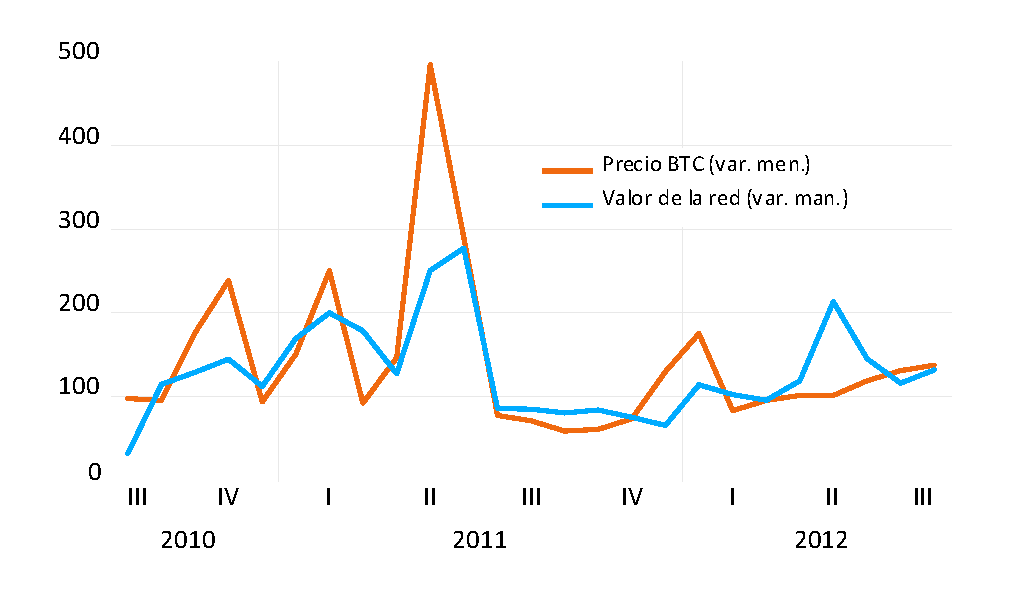
\includegraphics[width=1\textwidth]{images/C2/c2_var_men_timesseries_presentacion.pdf}
     \end{center}
\end{figure}

\note{
\begin{itemize}
    \item Luego de generar la serie temporal, se toma la serie en variaciones para dar cuenta del crecimiento poblacional "n". 
\end{itemize}
}

\end{frame}
%----------

% comparación con referencias actuales

\begin{frame}
\frametitle{Estos resultados se encuentran asociados a nuevas métricas de mercado}

\begin{figure}[H]
    \begin{center}
         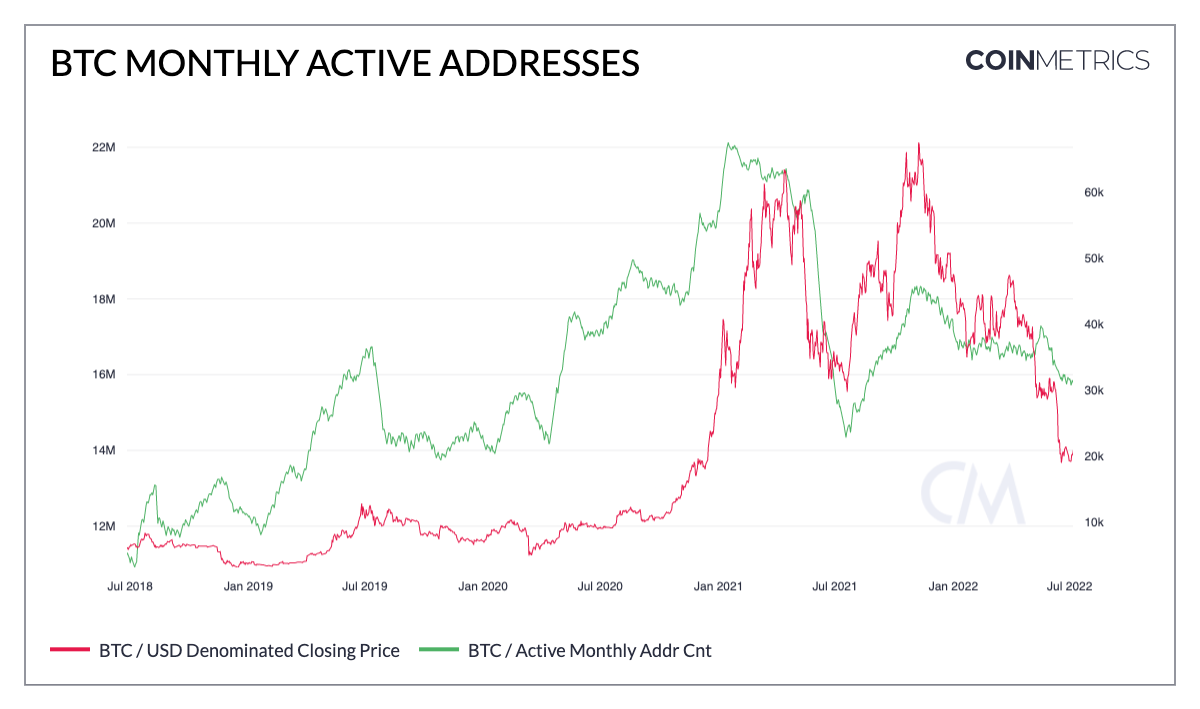
\includegraphics[width=1\textwidth]{images/C2/ref/coinmetrics_addr.png}
     \end{center}
\end{figure}

\note{
\begin{itemize}
    \item Este tipo de análisis a partir de datos de la cadena de bloques están comenzando a ser utilizados por consultoras de mercado para evaluar la evolución del precio de bitcoin y otros activos digitales. 
    \item Este es un indicador de la empresa Glassnode, donde se asocian las nuevas direcciones utilizadas en la red bitcoin al valor de mercado del bitcoin. 
\end{itemize}
}

\end{frame}
%----------

\begin{frame}
\frametitle{Estos resultados se encuentran asociados a nuevas métricas de mercado}

\begin{figure}[H]
    \begin{center}
         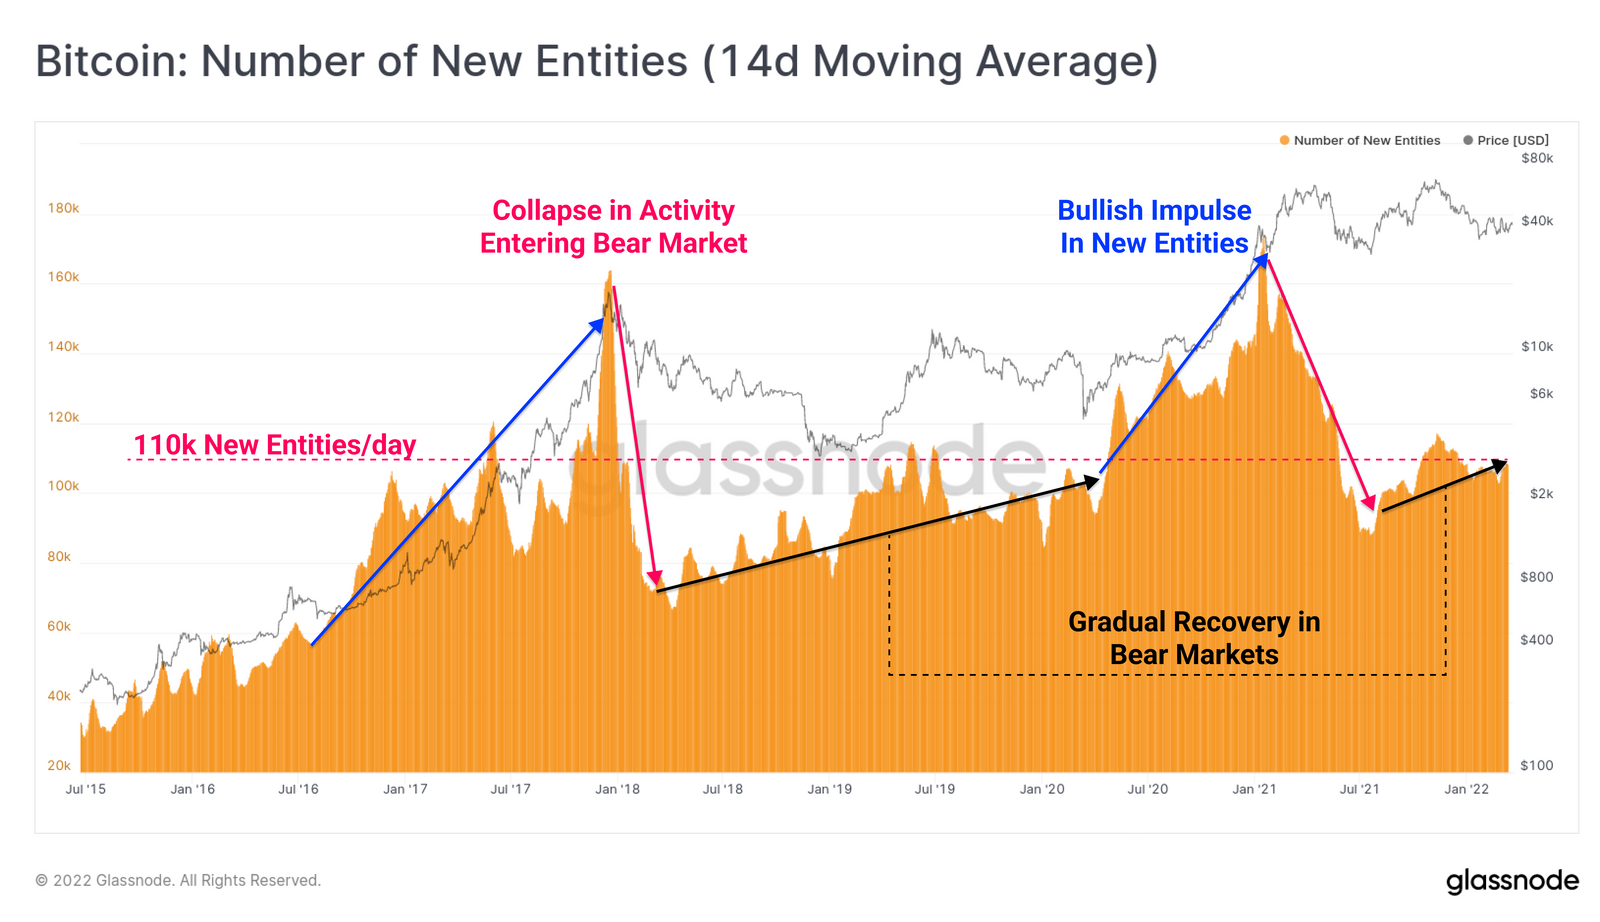
\includegraphics[width=1\textwidth]{images/C2/ref/07_newentities.png}
     \end{center}
\end{figure}

\note{
\begin{itemize}
    \item Este tipo de análisis a partir de datos de la cadena de bloques están comenzando a ser utilizados por consultoras de mercado para evaluar la evolución del precio de bitcoin y otros activos digitales. 
    \item Este es un indicador de la empresa Glassnode, donde se asocian las nuevas direcciones utilizadas en la red bitcoin al valor de mercado del bitcoin. 
\end{itemize}
}

\end{frame}
%----------

\begin{frame}{}

    \vspace{5mm}
    \begin{itemize}
        \setlength\itemsep{1em}
        \item[] La \textcolor{blue}{\textbf{conclusión principal}} es que \textcolor{blue}{bitcoin es una tecnología funcionalmente equivalente al dinero}.  
        \item[] La \textcolor{dgreen}{\textbf{evaluación conceptual}} corrobora la conjetura a partir de la introducción de la DLT en el modelo de generaciones superpuestas de manera directa como un \textcolor{dgreen}{sistema de registros público} y como \textcolor{dgreen}{memoria}.
        \item[] La \textcolor{orange}{\textbf{evaluación empírica}} corrobora la conjetura a partir de la \textcolor{orange}{construcción de una cadena de operaciones que simula al modelo} teórico.
    \end{itemize}

\note{
\begin{itemize}
    \item Luego de realizar la evaluación conceptual y empírica en esta primera parte de la investigación, se  llega a las siguientes conclusiones: (leer filmina)
\end{itemize}
}
    
\end{frame}
%----------


%################
\section{C3. Demanda}
%################

%-----------------------------------------------------
\subsubsection{Perspectiva general de la investigación}
%-----------------------------------------------------

\begin{frame}
\frametitle{Perspectiva general}
%------------------------------
\begin{columns}

    \begin{column}{0.50\textwidth}
    \vspace{-5pt}
    \begin{block}{\textcolor{blue}{Oferta}}
        \begin{column}{0.1\textwidth}
        \vspace{-10pt} % estos espacios negativos son claves para alinear
            \tiny
            \begin{align*}
            c_{1,t}+\Phi_t \le y\\
            c_{2,t+1}\le\Phi_{t+1}^R\\
            N_{t-1}\textcolor{red}{x_t} \cdot \Phi_{t-1}^{\textbf{DLT}}=N_t(*)
            \end{align*}
        \end{column}
        \begin{column}{0.35\textwidth}  
            \begin{figure}[H]
            \begin{center}
             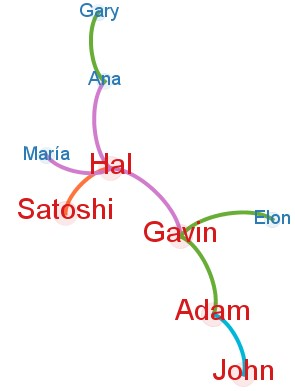
\includegraphics[width=1\textwidth]{images/C2/c2_simul_red5.jpg}
             \end{center}
            \end{figure}
            \end{column}
    \end{block}
    \begin{block}{\textcolor{dgreen}{Demanda}}
        \vspace{-10pt}
            \tiny
              \begin{align*}
              v_{t}^{\$}{M_{t}^{\$}}&={N_{t}^{\$}\left(*\right)}+(1-\lambda_t){N_{t}^{\$}\left(*\right)}\\
              v_{t}^{\bitcoinA}{M_{t}^{\bitcoinA}}&={N_{t}^{\bitcoinA}\left(*\right)+\lambda_tN_{t}^{\$}\left(*\right)}\\
              \lambda_t&=\textcolor{blue!70}{S}(\textcolor{red}{\mu_t})
            \end{align*}
    \vspace{-20pt}
            \begin{figure}[t!]
            \begin{center}
            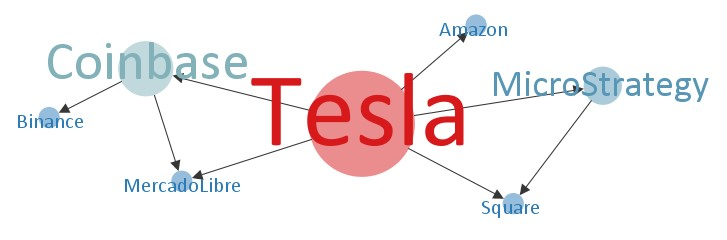
\includegraphics[width=0.6\textwidth]{images/C3/c3_simul_influ3.jpg}
             \end{center}
            \end{figure}
            
    \end{block}
    \end{column}
    
    \begin{column}{0.55\textwidth}
    
    \begin{block}{\textcolor{orange}{Implicancias}}
    \tiny

    \begin{align*}
    v^{\$a}_1 M^{\$a}_1&=P_1^{{\$a}} + \lambda_1 (1-\alpha_1) R_1^{{\$a}} + (1-\lambda_1) \textcolor{blue!60}{\rho_1}  R_1^{{\$a}}\\
    v_1^{\$} M_1^{\$}&=(1-\lambda_1) \textcolor{green!70}{\delta_1} R_1^{\$a}\\
    v_1^{\bitcoinA} M_1^{\bitcoinA}&=\textcolor{orange}{\lambda_1}  \alpha_1 R_1^{\$a} + (1-\lambda_1) \textcolor{red}{\beta_1} R_1^{\$a}\\
    e_t^{{\$a};{\$}}&=\frac{v_1^{\$a}}{v_1^{\$}}
    \end{align*}
    
    \vspace{-5pt}
    
    \begin{figure}[H]
    \begin{center}
     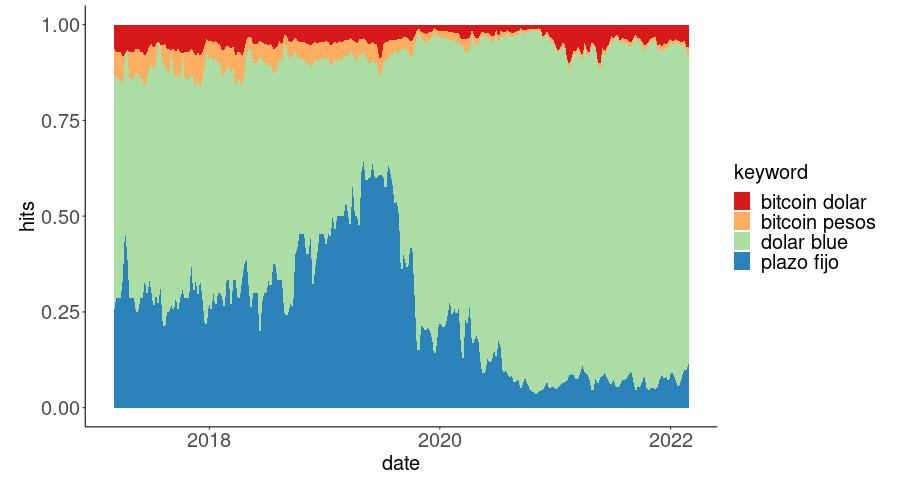
\includegraphics[width=1\textwidth]{images/C4/Rplot001.png}
     \end{center}
    \end{figure}
    
    \end{block}

    \end{column}
\end{columns}

\note{
\begin{itemize}
    \item Para poder dar respuestas a cada una de dichas preguntas se propone una evaluación conceptual y una evaluación empírica. 
    \item Evaluación conceptual
        \begin{itemize}
        \item Modelos OLG para los tres objetivos, con el mismo entorno (previsión perfecta, estacionariedad, un solo bien, dos generaciones que viven dos períodos, tiempo infinito).
        \end{itemize}
    \item Evaluación empírica
        \begin{itemize}
        \item Objetivo 1 y 2: técnicas de análisis de red
        \item Objetivo 3: datos de Google Trend (no hay posibilidad de georeferenciar datos de la blockchain o Twitter).
        \end{itemize}
\end{itemize}
}

\end{frame}
%----------
\addtocounter{framenumber}{-1}
\begin{frame}[plain]
\frametitle{Perspectiva general}
%------------------------------
\begin{columns}

    \pgfsetfillopacity{0.2}

    \begin{column}{0.50\textwidth}
    \vspace{-5pt}
    \begin{block}{\textcolor{cyan}{Oferta}}
        \begin{column}{0.1\textwidth}
        \vspace{-10pt} % estos espacios negativos son claves para alinear
            \tiny
            \begin{align*}
            c_{1,t}+\Phi_t \le y\\
            c_{2,t+1}\le\Phi_{t+1}^R\\
            N_{t-1}\textcolor{red}{x_t} \cdot \Phi_{t-1}^{\textbf{DLT}}=N_t(*)
            \end{align*}
        \end{column}
        \begin{column}{0.35\textwidth}  
            \begin{figure}[H]
            \begin{center}
             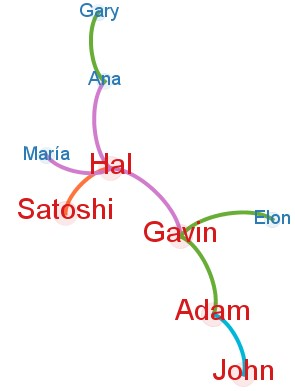
\includegraphics[width=1\textwidth]{images/C2/c2_simul_red5.jpg}
             \end{center}
            \end{figure}
            \end{column}
    \end{block}
    
    \pgfsetfillopacity{1}
    
    \begin{block}{\textcolor{dgreen}{Demanda}}
        \vspace{-10pt}
            \tiny
              \begin{align*}
              v_{t}^{\$}{M_{t}^{\$}}&={N_{t}^{\$}\left(*\right)}+(1-\lambda_t){N_{t}^{\$}\left(*\right)}\\
              v_{t}^{\bitcoinA}{M_{t}^{\bitcoinA}}&={N_{t}^{\bitcoinA}\left(*\right)+\lambda_tN_{t}^{\$}\left(*\right)}\\
              \lambda_t&=\textcolor{blue!70}{S}(\textcolor{red}{\mu_t})
            \end{align*}
    \vspace{-20pt}
            \begin{figure}[t!]
            \begin{center}
            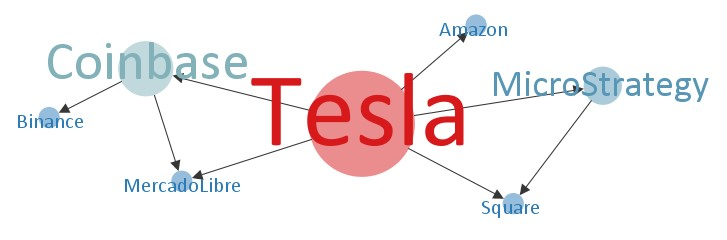
\includegraphics[width=0.6\textwidth]{images/C3/c3_simul_influ3.jpg}
             \end{center}
            \end{figure}
            
    \end{block}
    \end{column}
    
    \begin{column}{0.55\textwidth}
    
    \pgfsetfillopacity{0.2}
    
    \begin{block}{Implicancias}
    \tiny

    \begin{align*}
    v^{\$a}_1 M^{\$a}_1&=P_1^{{\$a}} + \lambda_1 (1-\alpha_1) R_1^{{\$a}} + (1-\lambda_1) \textcolor{blue!60}{\rho_1}  R_1^{{\$a}}\\
    v_1^{\$} M_1^{\$}&=(1-\lambda_1) \textcolor{green!70}{\delta_1} R_1^{\$a}\\
    v_1^{\bitcoinA} M_1^{\bitcoinA}&=\textcolor{orange}{\lambda_1}  \alpha_1 R_1^{\$a} + (1-\lambda_1) \textcolor{red}{\beta_1} R_1^{\$a}\\
    e_t^{{\$a};{\$}}&=\frac{v_1^{\$a}}{v_1^{\$}}
    \end{align*}
    
    \vspace{-5pt}
    
    \begin{figure}[H]
    \begin{center}
     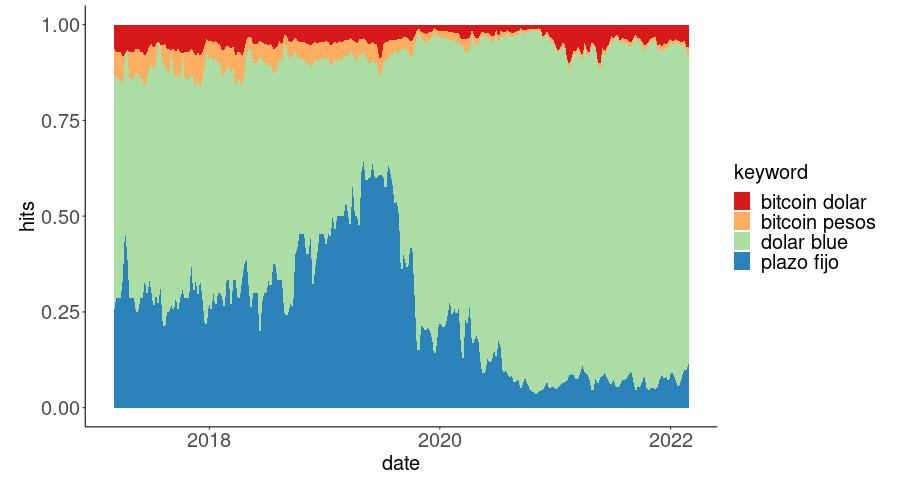
\includegraphics[width=1\textwidth]{images/C4/Rplot001.png}
     \end{center}
    \end{figure}
    
    \pgfsetfillopacity{1}
    
    \end{block}

    \end{column}
\end{columns}

\note{
\begin{itemize}
    \item Finalizada la primera parte de la investigación, volvemos a la filmina que presenta el panorama general. 
    \item Comenzamos con el análisis de la segunda parte de la investigación asociado a los motivos de demanda de bitcoin. 
\end{itemize}
}

\end{frame}
%----------

\subsection{Objetivos}
%---------------------
\begin{frame}{}

    \textcolor{blue}{\textbf{Objetivo}}.\\
    \vspace{5mm}
    \begin{itemize}
        \setlength\itemsep{1em}
        \item[] Analizar los \textcolor{blue}{motivos de demanda} de bitcoin. 
        \item[] Construir un \textcolor{blue}{modelo} que explique la demanda de bitcoin a partir del comportamiento de un grupo de \textcolor{blue}{influenciadores} y de un grupo de \textcolor{blue}{seguidores}. 
        \item[] Evaluar empíricamente el modelo propuesto a partir de \textcolor{blue}{datos estimados de las redes sociales}. 
    \end{itemize}
 
    \vspace{5mm}
    \textcolor{dgreen}{\textbf{Conjetura}}. 
    \vspace{5mm}
    \begin{itemize}
    \item[] La \textcolor{dgreen}{demanda de bitcoin} \textcolor{dgreen}{se encuentra asociada} de las opiniones de un grupo de \textcolor{dgreen}{actores influyentes} del mercado, de la opinión de los reguladores y del comportamiento de un grupo de seguidores. 
    \end{itemize}


\note{
\begin{itemize}
    \item Para esta segunda parte de la investigación, se plantean tres objetivos específicos
    \item (Leer cada objetivo)
    \item A su vez, se plantea la siguiente conjetura:
    \item (Leer la conjetura)
\end{itemize}
}
    
\end{frame}
%----------

\subsection{Definiciones}
%------------------------
\begin{frame}

\begin{displayquote}
\small
Las \textcolor{blue}{creencias} son importantes; si los jóvenes de un determinado período renuncian a algo de sus bienes por dinero, es porque piensan que la siguiente generación también lo hará.
\end{displayquote}
\raggedleft {\cite{Garratt2018},\\ \citetitle{Garratt2018}}

\vspace{5mm}
\begin{block}<2>{Creencias}
La demanda de un activo como activo monetario depende de las \textcolor{blue}{expectativas} en torno a que dicho activo pueda cumplir en el futuro con las \textcolor{blue}{funciones de medio de pago, reserva de valor y unidad de cuenta}. 
\end{block}

\note{
\begin{itemize}
    \item Para esta segunda parte de la investigación se propone retomar algunos conceptos asociados al valor del dinero fiduciario.
    \item En este sentido, \textbf{Garrat y Wallace} indican que (leer cita)
    \item A partir de esa definición, se propone el siguiente concepto de creencias (leer el recurado sobre DLT)
    \item En este sentido, por un lado, bitcoin se asemeja a las formas de dinero fiduciario actuales (como se indicó en la primera parte de la investigación). 
    \item Y, por otro, bitcoin se diferencia de los activos monetarios con valor intrínseco, como el oro, cuya demanda se encuentra vinculada, además, a su utilidad como bien de uso. 
\end{itemize}
}
    
\end{frame}
%----------

\begin{frame}

\begin{displayquote}
\small
Nada puede haber sido tan favorable a la génesis de un medio de cambio como la aceptación, por parte de \textcolor{blue}{los sujetos económicos más perspicaces y capaces}, para su propio beneficio económico, y durante un período de tiempo considerable, de bienes eminentemente vendibles con preferencia a todos los demás. 
\end{displayquote}
\raggedleft \href{https://www.jstor.org/stable/2956146}{\cite{Menger1892},\\ \citetitle{Menger1892},\\Sección VI}

\vspace{5mm}
\begin{block}<2>{Infuenciadores}
Los \textcolor{dgreen}{influenciadores} son \textcolor{blue}{actores} que \textcolor{blue}{generan información} nueva. Son actores que cuentan con \textcolor{blue}{más información} y \textcolor{blue}{mejor capacidad de análisis} que el resto de los demandantes del mercado. Son quienes determinan la tendencia de precios en el largo plazo. 
\end{block}

\note{
\begin{itemize}
    \item Una segunda idea relevante para esta segunda parte de la investigación es la que distingue a ciertos grupos por sobre el resto al momento de determinar que activos funcionarán como medios de intercambio. 
    \item En este sentido, por ejemplo, Menger, en una publicación muy influyente sobre el origen del dinero indica que (leer cita).
    \item A partir de estas ideas de Menger, se propone definir a los actores influyentes como (leer recuadro)
\end{itemize}
}
    
\end{frame}
%----------

\begin{frame}

\begin{displayquote}
La sabiduría mundana enseña que es mejor para la \textcolor{blue}{reputación} \textcolor{blue}{fracasar convencionalmente} que tener éxito de forma no convencional.
\end{displayquote}
\raggedleft \cite{Keynes1936TheExpectation} \\ \citetitle{Keynes1936TheExpectation}\\ Sección V

\vspace{5mm}
\begin{block}<2>{Seguidores}
Los \textcolor{dgreen}{seguidores} son los agentes que \textcolor{blue}{imitan} el comportamiento de los actores influyentes. El comportamiento de los seguidores se encuentra asociado al comportamiento en el precio de corto plazo. 
\end{block}

\note{
\begin{itemize}
    \item Finalmente, otra idea relevante para esta segunda parte de la investigación se asocia al comportamiento de actores imitadores.  
    \item En este sentido, por ejemplo, Keynes, en la última parte de la sección 5 del capítulo 12 de Teoría General (sección donde se desarrollan las ideas del concurso de belleza) indica que (leer cita).
    \item A partir de estas ideas de Keynes, se propone definir a los seguidores como (leer recuadro)
\end{itemize}
}
    
\end{frame}
%----------

\subsection{Evaluación conceptual y empírica}
%-----------------------------------------------

% overview
\begin{frame}{Evaluación conceptual y empírica}
    
    \begin{block}{Modelo}
    
    \begin{minipage}[t][.20\textheight][t]{\textwidth}

        \begin{column}{0.30\textwidth}
            \tiny
            \begin{align*}
            v_{t}^{\$}{M_{t}^{\$}}&=     N_{t}^{\$}(y_{t}^{\$}-c_{t}^{\$})
            (1-\lambda_t)\\
            v_{t}^{\bitcoinA}{M_{t}^{\bitcoinA}}&=N_{t}^{\bitcoinA}(y_{t}^{\bitcoinA}-c_{t}^{\bitcoinA})+{N_{t}^{\$}(y_{t}^{\$}-c_{t}^{\$})}\lambda_t\\
            {\lambda_t}&={S}({\mu_t})
            \end{align*}
        \end{column}
        \begin{column}{0.45\textwidth}
        
        \end{column}
        
    \end{minipage}
    \end{block}

\begin{block}{Evaluación empírica}
    
    \begin{minipage}[t][.40\textheight][t]{\textwidth}

\begin{column}{0.3\textwidth}
    \tiny
    \begin{figure}[H]
        \begin{center}
             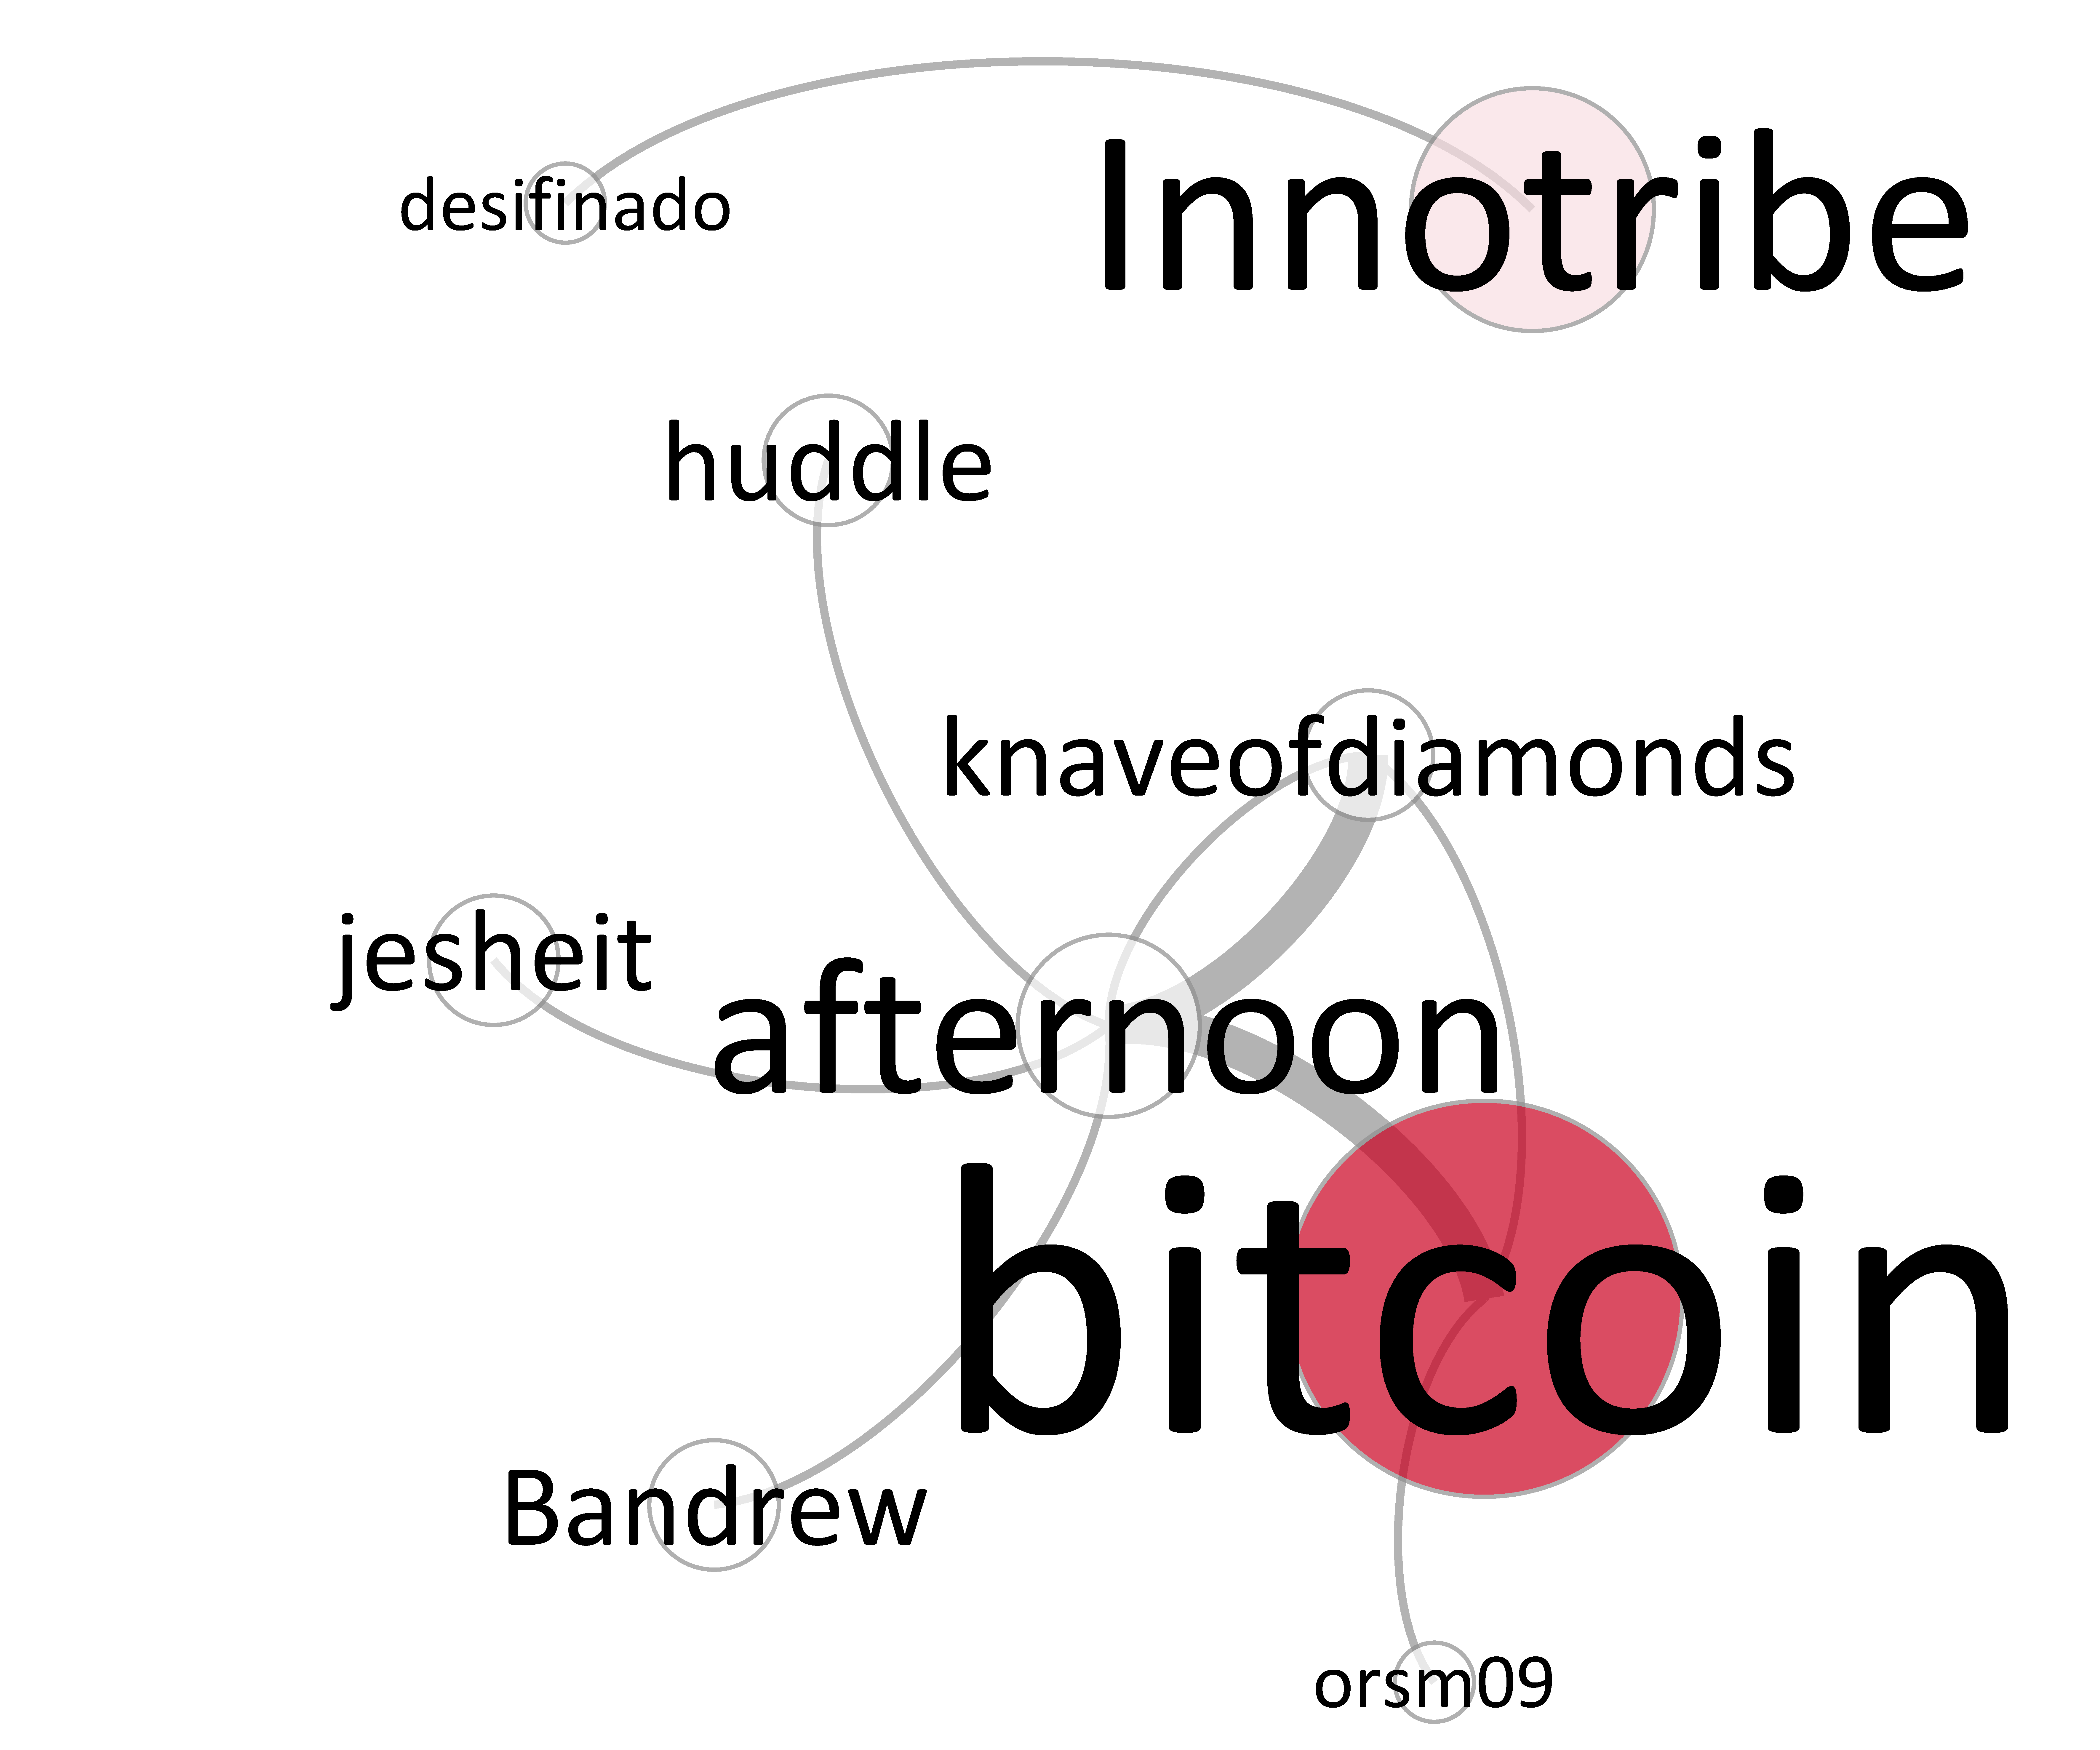
\includegraphics[width=1\textwidth]{images/C3/c3_red_influ_real.pdf}
         \end{center}
    \end{figure}
\end{column}
\begin{column}{0.3\textwidth}  
    \tiny
    \begin{figure}[H]
        \begin{center}
         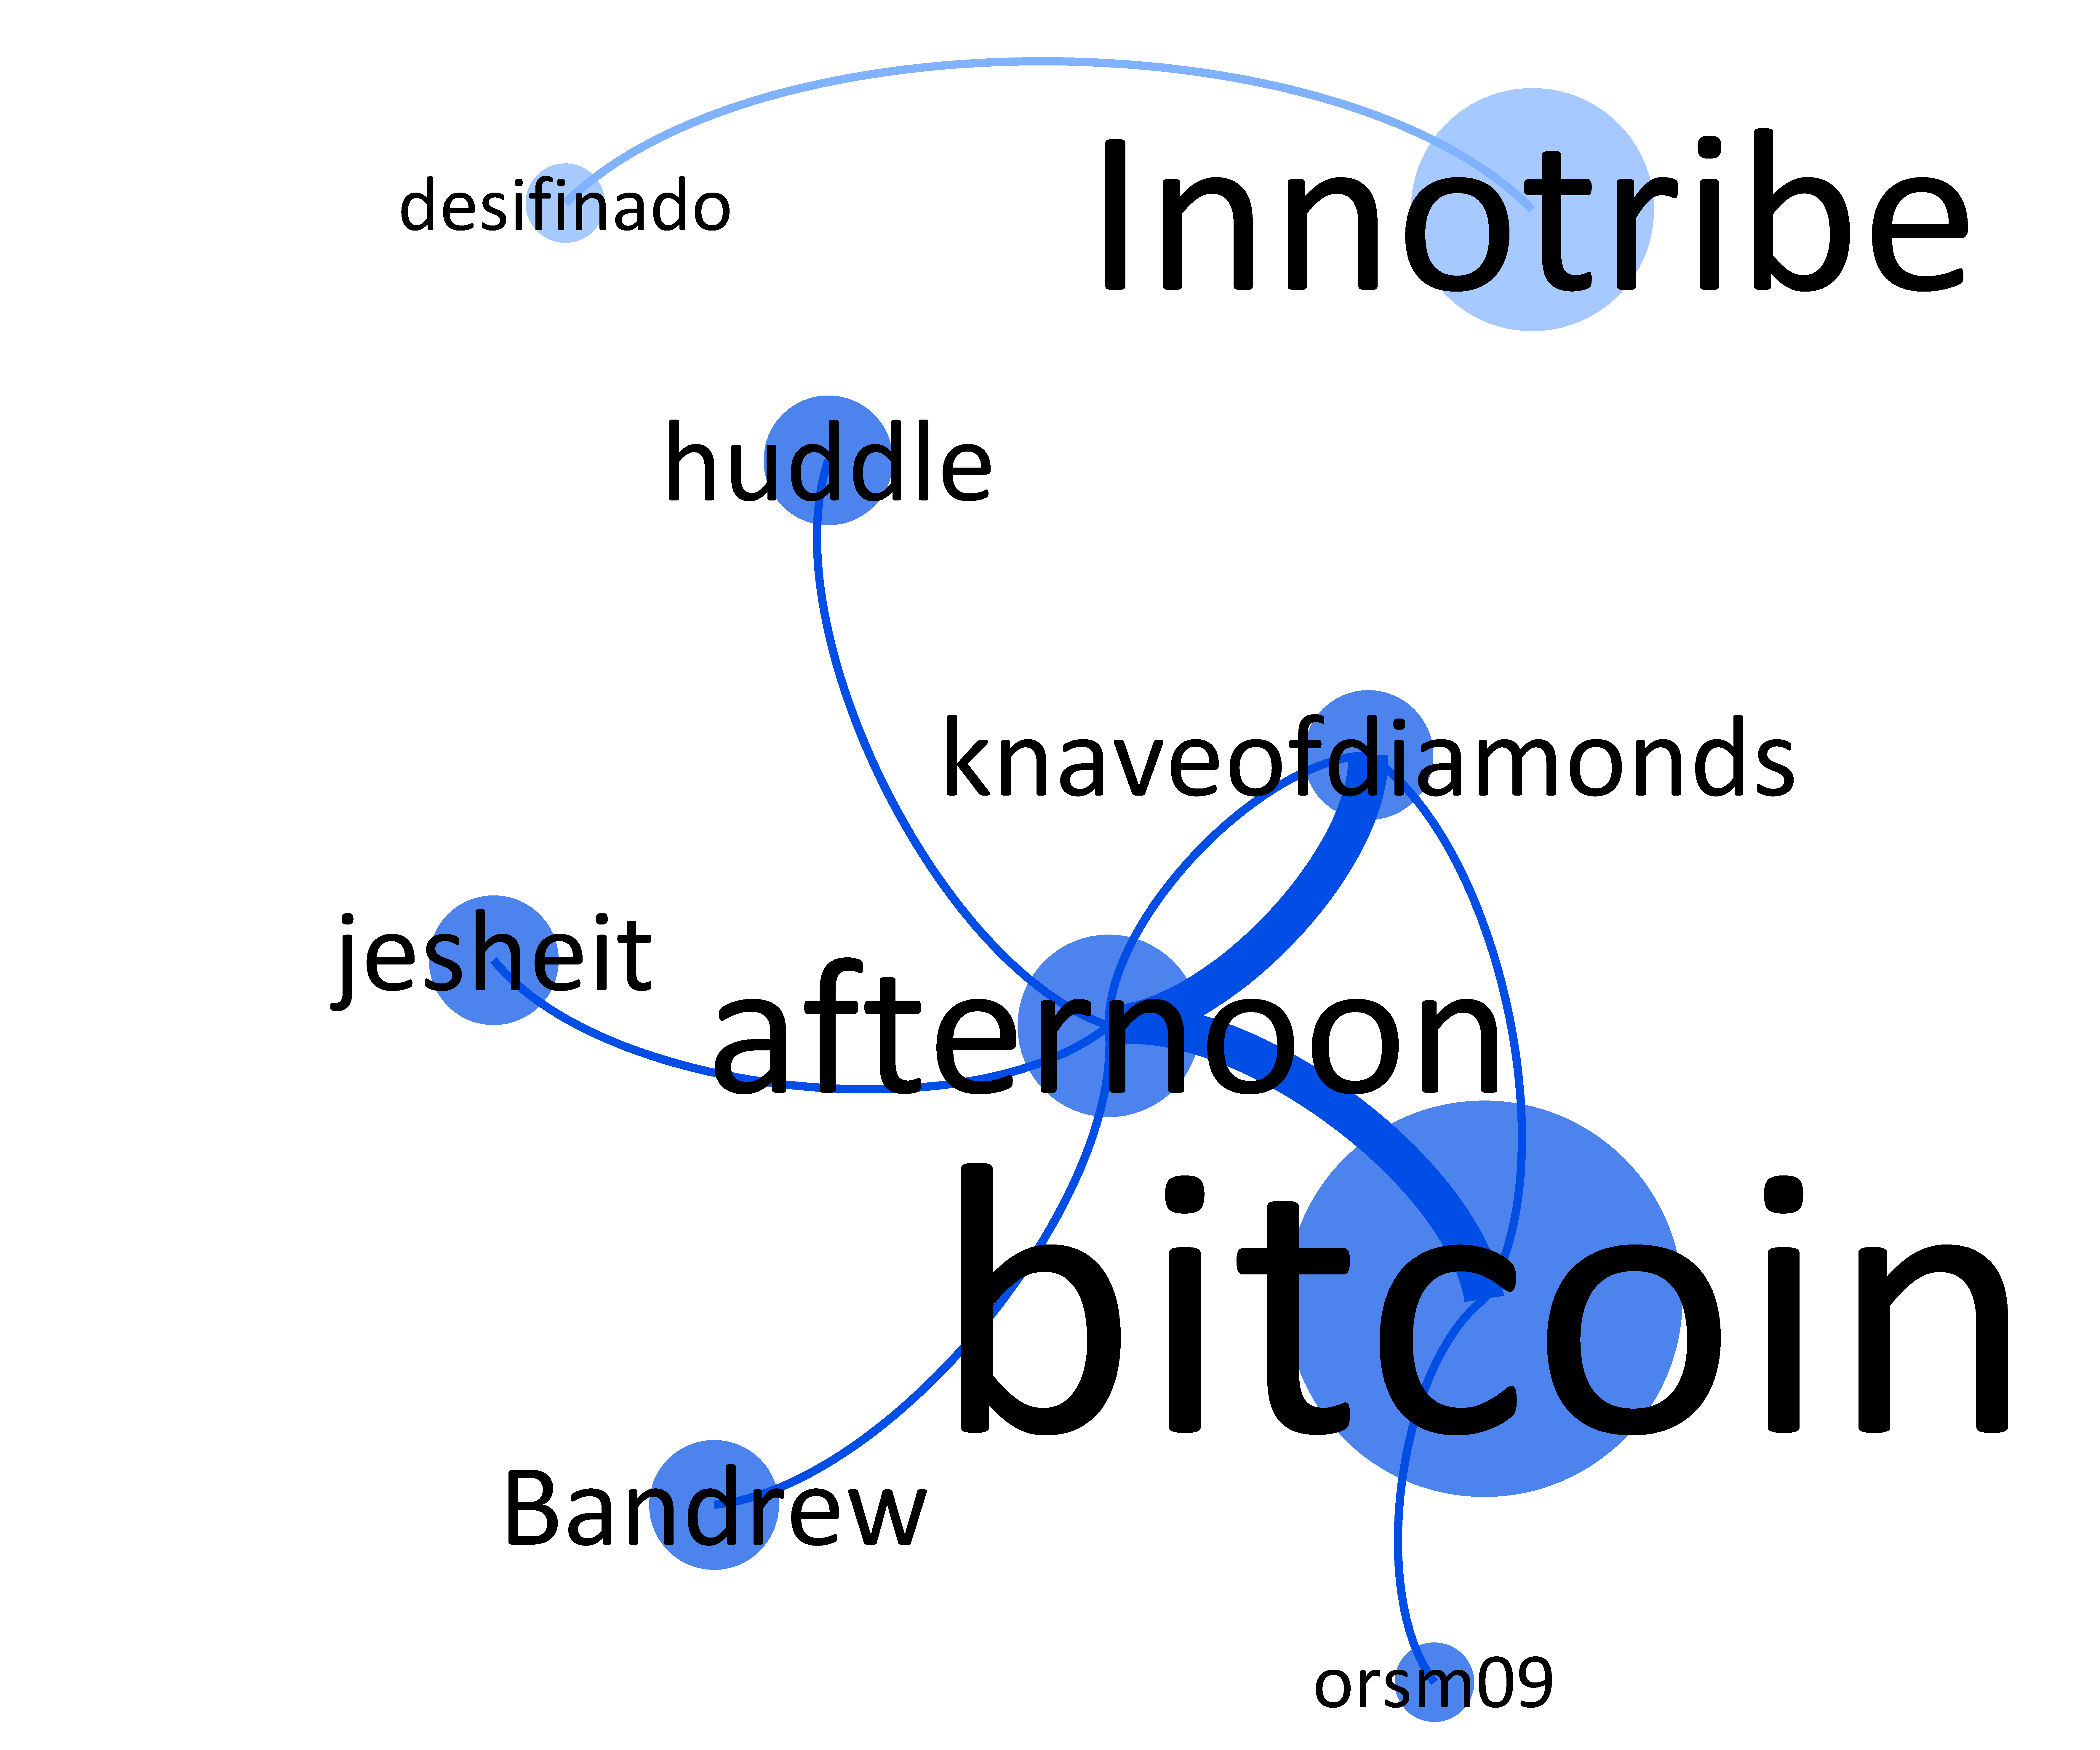
\includegraphics[width=1\textwidth]{images/C3/c3_red_comunidades_real.pdf}
         \end{center}
    \end{figure}
\end{column}
\begin{column}{0.3\textwidth}  
    \tiny
    \begin{figure}[H]
        \begin{center}
         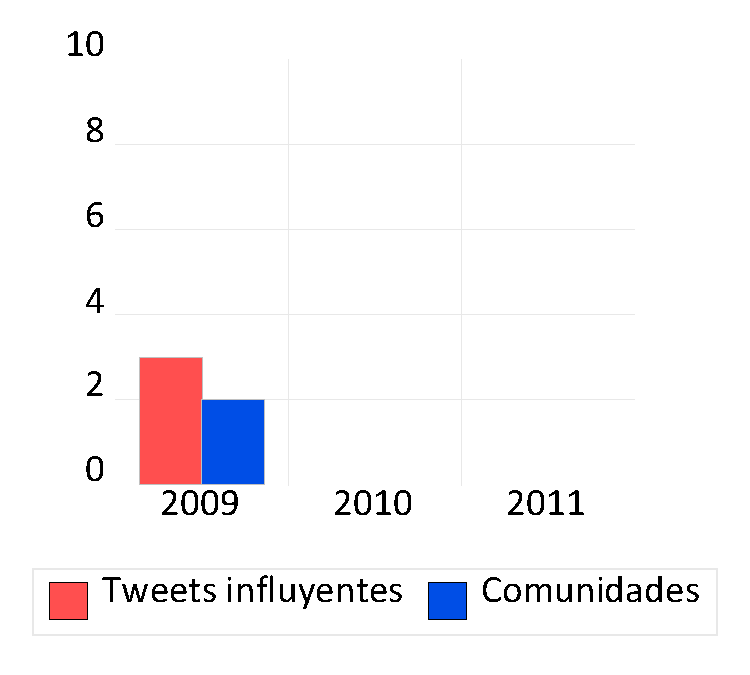
\includegraphics[width=1\textwidth]{images/C3/c3_timesseries_2009_real.pdf}
         \end{center}
    \end{figure}
\end{column}

    \end{minipage}

\end{block}

\note{
\begin{itemize}
    \item Para esta segunda parte de la investigación se propone: 
    \item Evaluación conceptual: modelo generaciones superpuestas con dos activos monetarios (dinero fiduciario y bitcoin) y dos actores (influyentes y seguidores). 
    \item De manera alternativa, se propone una explicación desde la teoría de juegos con un juego simultáneo con información perfecta. En este juego existe la posibilidad de equilibrios múltiples bajo problemas de coordinación. El análisis desde la teoría de juegos se encuentra en el anexo GameTheory.
    \item Evaluación empírica: análisis con técnicas de red a partir de mensajes de la red social twitter
    \end{itemize}
}

\end{frame}
% slides del modelo con overlay

\begin{frame}[t]
\frametitle{Evaluación conceptual y empírica}
    
    \begin{block}{Modelo}
    
    \begin{minipage}[t][.20\textheight][t]{\textwidth}

        \begin{column}{0.30\textwidth}
            \tiny
            \begin{align*}
            \onslide<2,4>{v_{t}^{\$}{M_{t}^{\$}}}&=      \onslide<3,4,6>{N_{t}^{\$}(y_{t}^{\$}-c_{t}^{\$})}\onslide<6>{(1-\lambda_t)}\\
            \onslide<5>{v_{t}^{\bitcoinA}{M_{t}^{\bitcoinA}}}&=
            \onslide<5>{N_{t}^{\bitcoinA}(y_{t}^{\bitcoinA}-c_{t}^{\bitcoinA})}+
            \onslide<6>{{N_{t}^{\$}(y_{t}^{\$}-c_{t}^{\$})}\onslide<6>{\lambda_t}}\\
            \only<7|handout:0>{{\lambda_t}&={S}({\mu_t})}
            \only<8>{{\lambda_t}&={S}(\textcolor{red}{\mu_t})}
            \only<9|handout:0>{{\lambda_t}&=\textcolor{blue!70}{S}({\mu_t})}
            \end{align*}
        \end{column}
        \begin{column}{0.45\textwidth}
        \only<2|handout:0>{
                    \tiny
                    \justify
                    Oferta de dinero fiduciario
                    \begin{itemize}
                        \item $v_t^{\$}$: valor de una unidad del act
                        ivo fiduciario en término de bienes;
                        \item $M_t^{\$}$: oferta de activo fiduciario.
                    \end{itemize}
                    }
        
        \only<3|handout:0>{
                    \tiny
                    \justify
                    Demanda de dinero fiduciario
                    \begin{itemize}
                        \item $y_t^{\$}$: asignación de bienes
                        \item $c_t^{\$}$: consumo
                        \item $N_t^{\$}$: cantidad de personas
                    \end{itemize}
                    }
                    
        \only<4|handout:0>{
                    \tiny
                    \justify
                    Mercado de dinero fiduciario
                    }

        \only<5|handout:0>{
                    \tiny
                    \justify
                    Mercado de dinero criptográfico
                    }
        
        \only<6|handout:0>{
                    \tiny
                    \justify
                    Sustititución monetaria
                    }
        
        \only<7|handout:0>{
                    \tiny
                    \justify
                    Parámetro de grado de influencia
                    \begin{itemize}
                        \item $\mu_t$ influenciadores
                        \item $S$ seguidores
                    \end{itemize}
                    }
        
        \only<8>{
                    \tiny
                    \justify
                    Parámetro de grado de influencia
                    \begin{itemize}
                        \item $\mu_t$ \textcolor{red}{influenciadores}
                        \item $S$ seguidores
                    \end{itemize}
                    }
                    
        
        \only<9|handout:0>{
                    \tiny
                    \justify
                    Parámetro de grado de influencia
                    \begin{itemize}
                        \item $\mu_t$ influenciadores
                        \item $S$ \textcolor{blue!70}{seguidores}
                    \end{itemize}
                    }
        
        \end{column}
        
    \end{minipage}
    \end{block}

\begin{block}{Evaluación empírica}

\begin{minipage}[t][.40\textheight][t]{\textwidth}
    
\begin{column}{0.3\textwidth}
    \tiny
    \begin{figure}[H]
        \begin{center}
             \includegraphics<8,9>[width=1\textwidth]{images/C3/c3_red_influ_real.pdf}
         \end{center}
    \end{figure}
\end{column}
\begin{column}{0.3\textwidth}  
    \tiny
    \begin{figure}[H]
        \begin{center}
         \includegraphics<9>[width=1\textwidth]{images/C3/c3_red_comunidades_real.pdf}
         \end{center}
    \end{figure}
\end{column}
\begin{column}{0.3\textwidth}  
    \tiny
    \begin{figure}[H]
        \begin{center}
         \includegraphics<8|handout:0>[width=1\textwidth]{images/C3/c3_timesseries_2009_real_v02.pdf}
        \includegraphics<9>[width=1\textwidth]{images/C3/c3_timesseries_2009_real.pdf}
         \end{center}
    \end{figure}
\end{column}

\end{minipage}
\end{block}

\note{
\small
\begin{itemize}
    \item 1° Economía con un activo monetario fiduciario.
    \item 2° Creación de una nueva moneda digital. Uso limitado
    \item 3° Sustitución 
    \item De la fracción de ciudadanos que elija el activo digital y, por lo tanto, el activo fiduciario, estará asociada al comportamiento de un grupo de actores influyentes y de un grupo de seguidores
    \item Se define, por lo tanto, el parámetro de grado de influencia como: $\lambda_t=S(\mu_t)$; $\mu_t$: parámetro interés del grupo de actores influyentes; $S$ función indica comportamiento de imitación de seguidores. El parámetro $\mu_t$ depende, a su vez, del interés de actores influyentes de mercado y del regulador. La función $S$ amplifica el interés reflejado por parte de los influenciadores. 
\end{itemize}
}

\end{frame}

% slides de evaluación empírica 2010 2 de 2

\begin{frame}[t]
\frametitle{Evaluación conceptual y empírica}
    
    \begin{block}{Modelo}
    
    \begin{minipage}[t][.20\textheight][t]{\textwidth}

        \begin{column}{0.30\textwidth}
            \tiny
            \begin{align*}
            v_{t}^{\$}{M_{t}^{\$}}&=     N_{t}^{\$}(y_{t}^{\$}-c_{t}^{\$})
            (1-\lambda_t)\\
            v_{t}^{\bitcoinA}{M_{t}^{\bitcoinA}}&=N_{t}^{\bitcoinA}(y_{t}^{\bitcoinA}-c_{t}^{\bitcoinA})+{N_{t}^{\$}(y_{t}^{\$}-c_{t}^{\$})}\lambda_t\\
            {\lambda_t}&={S}({\mu_t})
            \end{align*}
        \end{column}
        \begin{column}{0.45\textwidth}
        
        \end{column}
        
    \end{minipage}
    \end{block}

\begin{block}{Evaluación empírica}

\begin{minipage}[t][.40\textheight][t]{\textwidth}
    
\begin{column}{0.3\textwidth}
    \tiny
    \begin{figure}[H]
        \begin{center}
             \includegraphics[width=1\textwidth]{images/C3/c3_red_influ_real_2010.pdf}
         \end{center}
    \end{figure}
\end{column}
\begin{column}{0.3\textwidth}  
    \tiny
    \begin{figure}[H]
        \begin{center}
         \includegraphics[width=1\textwidth]{images/C3/c3_red_com_real_2010.pdf}
         \end{center}
    \end{figure}
\end{column}
\begin{column}{0.3\textwidth}  
    \tiny
    \begin{figure}[H]
        \begin{center}
         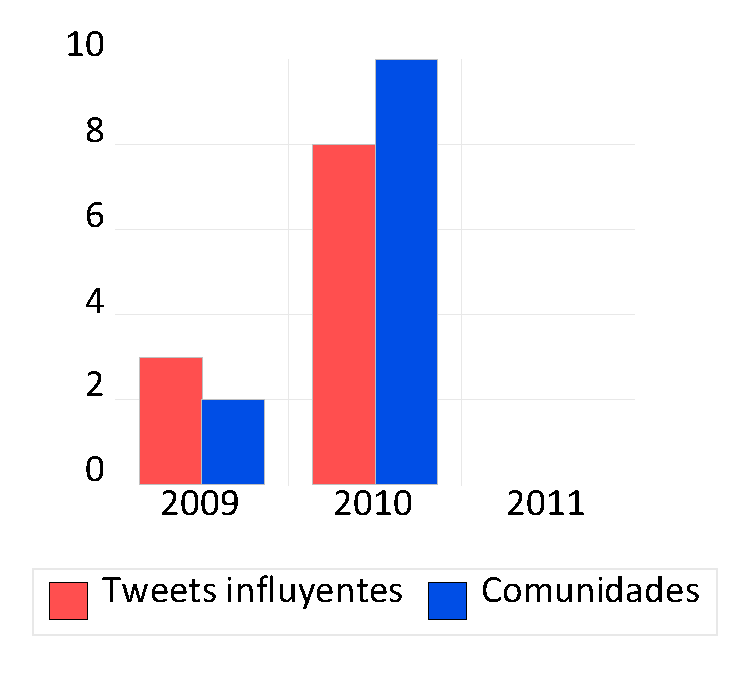
\includegraphics[width=1\textwidth]{images/C3/c3_times_series_2010.pdf}
         \end{center}
    \end{figure}
\end{column}

\end{minipage}
\end{block}

\note{
\footnotesize
\begin{itemize}
    \item La conjetura empírica indica que existe una asociación entre el valor de $\lambda$ y el valor del activo digital. 
    \item Se espera que niveles elevados de $\lambda$ estén asociados a incrementos en el valor del activo digital. 
    \item Fuente: la recopilación de datos de tweets se efectúa mediante Python
    \item Para generar la lista de \textbf{actores influyentes} (gráfico de la izq) se utiliza la métrica de pagerank que mide la importancia de cada nodo dentro del gráfico basándose en el número de relaciones entrantes y la importancia de los nodos fuente correspondientes. El supuesto subyacente es que un actor es tan importante como los actores con los que se conecta. 
    \item Para estimar el comportamiento de los \textbf{seguidores}, se estudian los mismos datos, la misma red, pero desde una dimensión diferente. Ahora se quiere evaluar la estructura de la red, su topología. Se considera que una red más densa debería propagar los mensajes de los influyentes con mayor velocidad y, por lo tanto, debería amplificar su sentido. 
\end{itemize}
}

\end{frame}
%----------

\subsection{Resultados}
%---------------------


\begin{frame}
\frametitle{Se compara la variación de \textcolor{red}{tweets influentes}...}

\begin{figure}[H]
    \begin{center}
         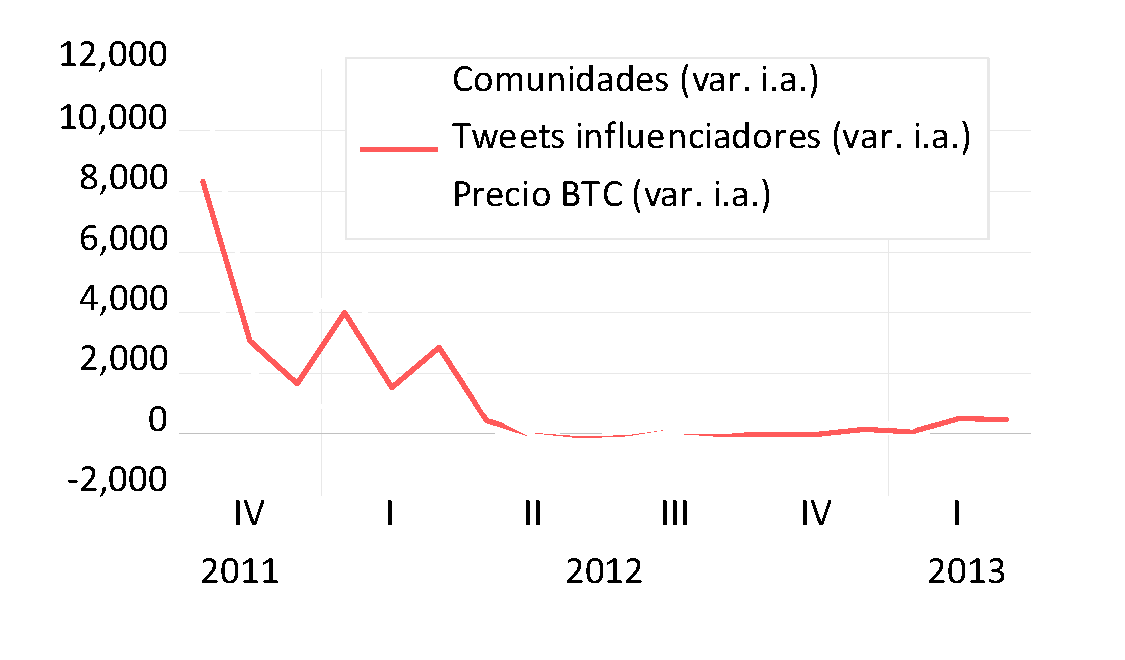
\includegraphics[width=1\textwidth]{images/C3/results/times_series_result_01.pdf}
     \end{center}
\end{figure}

\note{
\begin{itemize}
    \item Luego de estimar las variaciones asociadas a las opiniones de los actores influyentes a través del uso del algoritmo PageRank y estimar el comportamiento del grupo de seguidores a través de las métricas de red, se propone evaluar la asociación entre dichas estimaciones y el precio de bitcoin. Para estimar las relaciones entre variables se transforman las variables para obtener las variaciones interanuales. 
    \item (leer encabezado)
\end{itemize}
}

\end{frame}
%----------

\begin{frame}
\frametitle{...y la variación de \textcolor{blue}{comunidades}...}

\begin{figure}[H]
    \begin{center}
         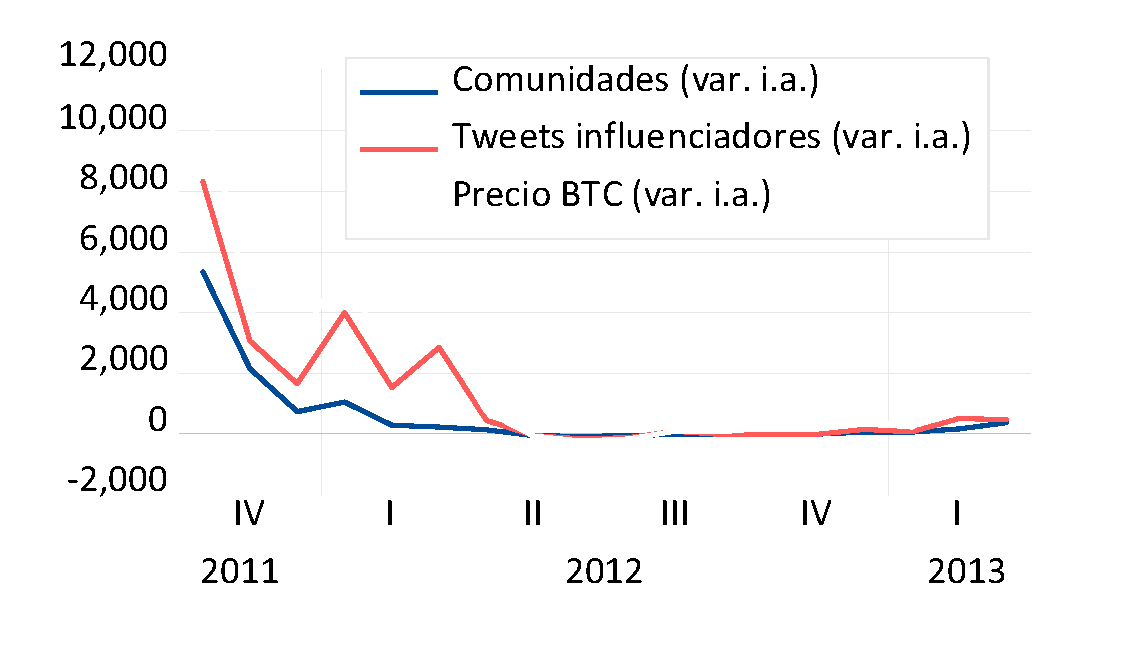
\includegraphics[width=1\textwidth]{images/C3/results/times_series_result_02.pdf}
     \end{center}
\end{figure}

\note{
\begin{itemize}
    \item (leer encabezado)
\end{itemize}
}

\end{frame}
%----------


\begin{frame}
\frametitle{con la variación en el \textcolor{dgreen}{precio}.}

\begin{figure}[H]
    \begin{center}
         \includegraphics[width=1\textwidth]{images/C3/results/times_series_result_03.pdf}
     \end{center}
\end{figure}

\note{
\begin{itemize}
    \item (leer encabezado)
    \item La correlación entre la variación i.a. del precio de bitcoin y la variación i.a. de los tweets de los influyentes es de 0.82 y la correlación entre la variación del precio de bitcoin y la variación i.a. de los nodos es 0.94.
\end{itemize}
}

\end{frame}
%----------

% comparación con referencias actuales

\begin{frame}
\frametitle{Estos resultados se encuentran asociados a nuevas métricas de mercado}

\begin{figure}[H]
    \begin{center}
         \includegraphics[width=1\textwidth]{images/C3/ref/reuters2.jpg}
     \end{center}
    \source{Fuente: \href{https://www.thomsonreuters.com/en/press-releases/2018/march/thomson-reuters-launches-bitcoin-sentiment-data-feed-for-trading-and-risk-management.html}{Thomson Reuters}}
\end{figure}

\note{
\begin{itemize}
    \item Este tipo de análisis a partir de datos de redes sociales están comenzando a ser utilizados por consultoras de mercado para evaluar la evolución del precio de bitcoin y otros activos digitales. 
    \item Este es un indicador de la empresa Thomson Reuters.
\end{itemize}
}

\end{frame}
%----------

\begin{frame}{}

    \vspace{5mm}
    \begin{itemize}
        \setlength\itemsep{1em}
        \item[] La \textcolor{blue}{\textbf{conclusión principal}} es que la \textcolor{blue}{demanda de bitcoin se encuentra asociada} del comportamiento de un grupo de actores \textcolor{blue}{influyentes} y un grupo de \textcolor{blue}{seguidores}.
        \item[] La \textcolor{dgreen}{\textbf{evaluación conceptual}} corrobora la conjetura a partir de la introducción en el modelo OLG la ecuación del \textcolor{dgreen}{parámetro de influencia ($\lambda$)} en función del comportamiento de un grupo de actores influyentes y del comportamiento de un grupo de seguidores. 
        \item[] La \textcolor{orange}{\textbf{evaluación empírica}} corrobora la conjetura a partir de la \textcolor{orange}{correlación} entre el \textcolor{orange}{precio} de bitcoin y los \textcolor{orange}{tweets} de los actores influyentes ponderados por la estructura de red asociada al comportamiento de los seguidores.   

    \end{itemize}

\note{
\begin{itemize}
    \item Luego de realizar la evaluación conceptual y empírica en esta segunda parte de la investigación, se  llega a las siguientes conclusiones: (leer filmina)
\end{itemize}
}
    
\end{frame}
%----------

%#####################
\section{C4. Implicancias}
%#####################

%-----------------------------------------------------
\subsubsection{Perspectiva general de la investigación}
%-----------------------------------------------------

\begin{frame}
\frametitle{Perspectiva general}
%------------------------------
\begin{columns}

    \begin{column}{0.50\textwidth}
    \vspace{-5pt}
    \begin{block}{\textcolor{blue}{Oferta}}
        \begin{column}{0.1\textwidth}
        \vspace{-10pt} % estos espacios negativos son claves para alinear
            \tiny
            \begin{align*}
            c_{1,t}+\Phi_t \le y\\
            c_{2,t+1}\le\Phi_{t+1}^R\\
            N_{t-1}\textcolor{red}{x_t} \cdot \Phi_{t-1}^{\textbf{DLT}}=N_t(*)
            \end{align*}
        \end{column}
        \begin{column}{0.35\textwidth}  
            \begin{figure}[H]
            \begin{center}
             \includegraphics[width=1\textwidth]{images/C2/c2_simul_red5.jpg}
             \end{center}
            \end{figure}
            \end{column}
    \end{block}
    \begin{block}{\textcolor{dgreen}{Demanda}}
        \vspace{-10pt}
            \tiny
              \begin{align*}
              v_{t}^{\$}{M_{t}^{\$}}&={N_{t}^{\$}\left(*\right)}+(1-\lambda_t){N_{t}^{\$}\left(*\right)}\\
              v_{t}^{\bitcoinA}{M_{t}^{\bitcoinA}}&={N_{t}^{\bitcoinA}\left(*\right)+\lambda_tN_{t}^{\$}\left(*\right)}\\
              \lambda_t&=\textcolor{blue!70}{S}(\textcolor{red}{\mu_t})
            \end{align*}
    \vspace{-20pt}
            \begin{figure}[t!]
            \begin{center}
            \includegraphics[width=0.6\textwidth]{images/C3/c3_simul_influ3.jpg}
             \end{center}
            \end{figure}
            
    \end{block}
    \end{column}
    
    \begin{column}{0.55\textwidth}
    
    \begin{block}{\textcolor{orange}{Implicancias}}
    \tiny

    \begin{align*}
    v^{\$a}_1 M^{\$a}_1&=P_1^{{\$a}} + \lambda_1 (1-\alpha_1) R_1^{{\$a}} + (1-\lambda_1) \textcolor{blue!60}{\rho_1}  R_1^{{\$a}}\\
    v_1^{\$} M_1^{\$}&=(1-\lambda_1) \textcolor{green!70}{\delta_1} R_1^{\$a}\\
    v_1^{\bitcoinA} M_1^{\bitcoinA}&=\textcolor{orange}{\lambda_1}  \alpha_1 R_1^{\$a} + (1-\lambda_1) \textcolor{red}{\beta_1} R_1^{\$a}\\
    e_t^{{\$a};{\$}}&=\frac{v_1^{\$a}}{v_1^{\$}}
    \end{align*}
    
    \vspace{-5pt}
    
    \begin{figure}[H]
    \begin{center}
     \includegraphics[width=1\textwidth]{images/C4/Rplot001.png}
     \end{center}
    \end{figure}
    
    \end{block}

    \end{column}
\end{columns}

\note{
\begin{itemize}
    \item Para poder dar respuestas a cada una de dichas preguntas se propone una evaluación conceptual y una evaluación empírica. 
    \item Evaluación conceptual
        \begin{itemize}
        \item Modelos OLG para los tres objetivos, con el mismo entorno (previsión perfecta, estacionariedad, un solo bien, dos generaciones que viven dos períodos, tiempo infinito).
        \end{itemize}
    \item Evaluación empírica
        \begin{itemize}
        \item Objetivo 1 y 2: técnicas de análisis de red
        \item Objetivo 3: datos de Google Trend (no hay posibilidad de georeferenciar datos de la blockchain o Twitter).
        \end{itemize}
\end{itemize}
}

\end{frame}
%----------
\addtocounter{framenumber}{-1}
\begin{frame}[plain]
\frametitle{Perspectiva general}
%------------------------------
\begin{columns}

    \pgfsetfillopacity{0.2}

    \begin{column}{0.50\textwidth}
    \vspace{-5pt}
    \begin{block}{\textcolor{blue}{Oferta}}
        \begin{column}{0.1\textwidth}
        \vspace{-10pt} % estos espacios negativos son claves para alinear
            \tiny
            \begin{align*}
            c_{1,t}+\Phi_t \le y\\
            c_{2,t+1}\le\Phi_{t+1}^R\\
            N_{t-1}\textcolor{red}{x_t} \cdot \Phi_{t-1}^{\textbf{DLT}}=N_t(*)
            \end{align*}
        \end{column}
        \begin{column}{0.35\textwidth}  
            \begin{figure}[H]
            \begin{center}
             \includegraphics[width=1\textwidth]{images/C2/c2_simul_red5.jpg}
             \end{center}
            \end{figure}
            \end{column}
    \end{block}
    
    \begin{block}{\textcolor{dgreen}{Demanda}}
        \vspace{-10pt}
            \tiny
              \begin{align*}
              v_{t}^{\$}{M_{t}^{\$}}&={N_{t}^{\$}\left(*\right)}+(1-\lambda_t){N_{t}^{\$}\left(*\right)}\\
              v_{t}^{\bitcoinA}{M_{t}^{\bitcoinA}}&={N_{t}^{\bitcoinA}\left(*\right)+\lambda_tN_{t}^{\$}\left(*\right)}\\
              \lambda_t&=\textcolor{blue!70}{S}(\textcolor{red}{\mu_t})
            \end{align*}
    \vspace{-20pt}
            \begin{figure}[t!]
            \begin{center}
            \includegraphics[width=0.6\textwidth]{images/C3/c3_simul_influ3.jpg}
             \end{center}
            \end{figure}
            
    \end{block}
    \end{column}
    
    \begin{column}{0.55\textwidth}
    
    \pgfsetfillopacity{1}
    
    \begin{block}{\textcolor{orange}{Implicancias}}
    \tiny

    \begin{align*}
    v^{\$a}_1 M^{\$a}_1&=P_1^{{\$a}} + \lambda_1 (1-\alpha_1) R_1^{{\$a}} + (1-\lambda_1){\rho_1}  R_1^{{\$a}}\\
    v_1^{\$} M_1^{\$}&=(1-\lambda_1) \textcolor{green!70}{\delta_1} R_1^{\$a}\\
    v_1^{\bitcoinA} M_1^{\bitcoinA}&={\lambda_1}  \alpha_1 R_1^{\$a} + (1-\lambda_1){\beta_1} R_1^{\$a}\\
    e_t^{{\$a};{\$}}&=\frac{v_1^{\$a}}{v_1^{\$}}
    \end{align*}
    
    \vspace{-5pt}
    
    \begin{figure}[H]
    \begin{center}
     \includegraphics[width=1\textwidth]{images/C4/Rplot001.png}
     \end{center}
    \end{figure}
    
    \end{block}

    \end{column}
\end{columns}

\note{
\begin{itemize}
    \item Finalizada la primera y segunda parte de la investigación, volvemos a la filmina que presenta el panorama general. 
    \item Ahora vamos a comenzar con la última parte de la investigación asociada a las implicancias de una mayor adopción de bitcoin en Argentina. 
\end{itemize}
}

\end{frame}
%----------

\subsection{Objetivos}
%---------------------
\begin{frame}{}

    \textcolor{blue}{\textbf{Objetivo}}.\\
    \vspace{5mm}
    \begin{itemize}
        \setlength\itemsep{1em}
        \item[] Analizar los riesgos para la estabilidad financiera asociados a bitcoin en una economía emergente. 
        \item[] Construir un \textcolor{blue}{modelo} que explique las consecuencias de un incremento en la \textcolor{blue}{volatilidad de demanda de bitcoin} en el nivel del \textcolor{blue}{tipo de cambio} entre pesos y dólares en Argentina.
        \item[] \textcolor{blue}{Evaluar empíricamente} el modelo propuesto a partir de datos estimados para Argentina.
    \end{itemize}
 
    \vspace{5mm}
    \textcolor{dgreen}{\textbf{Conjetura}}. 
    \vspace{5mm}
    \begin{itemize}
    \item[] Incrementos en la  \textcolor{dgreen}{volatilidad de la demanda de bitcoin} pueden generar incrementos en la  \textcolor{dgreen}{volatilidad en el tipo de cambio} entre pesos y dólares.
    \end{itemize}

\note{
\begin{itemize}
    \item Para esta tercera y última parte de la investigación, se plantean los siguientes tres objetivos específicos
    \item (Leer cada objetivo)
    \item A su vez, se plantea una última conjetura:
    \item (Leer la conjetura)
\end{itemize}
}
    
\end{frame}
%----------

\subsection{Definiciones}
%------------------------
\begin{frame}

\vspace{5mm}
\begin{displayquote}
\textcolor{blue}{Sustitución de monedas} se define como el uso en un país determinado de múltiples monedas como \textcolor{blue}{medio de cambio}. 
\end{displayquote}

\vspace{5mm}
\begin{displayquote}
El término \textcolor{dgreen}{dolarización} también se utiliza con frecuencia para indicar que una moneda extranjera sirve como unidad de cuenta o como \textcolor{dgreen}{depósito de valor}, y no necesariamente como medio de cambio.
\end{displayquote}
\vspace{5mm}
\raggedleft \cite{Calvo1992}\\ \citetitle{Calvo1992}

\note{
\begin{itemize}
    \item Para esta tercera parte de la investigación se propone retomar algunos conceptos asociados a la sustitución de activos monetarios.
    \item En este sentido, \textbf{Calvo y Vegh} proponen dos definiciones complementarias (leer citas)
    \item Esta distinción entre sustitución de activos como medios de pago o como reserva de valor será relevante para la presente parte de la investigación.  
\end{itemize}
}
    
\end{frame}
%----------

\subsection{Evaluación conceptual y empírica}
%-----------------------------------------------

% overwiew
\begin{frame}[t]
\frametitle{Evaluación conceptual y empírica}
    
    \begin{block}{Modelo}
        \vspace{-10pt}
        \begin{column}{0.4\textwidth}
            \tiny
            \begin{align*}
            v^{\$a}_1 M^{\$a}_1&=P_1^{{\$a}} + \lambda_1 (1-\alpha_1) R_1^{{\$a}} + (1-\lambda_1){\rho_1}  R_1^{{\$a}}\\
            v_1^{\$} M_1^{\$}&=(1-\lambda_1){\delta_1} R_1^{\$a}\\
            v_1^{\bitcoinA} M_1^{\bitcoinA}&={\lambda_1}  \alpha_1 R_1^{\$a} + (1-\lambda_1){\beta_1} R_1^{\$a}\\
            e_t^{{\$a};{\$}}&=\frac{v_1^{\$a}}{v_1^{\$}}
            \end{align*}
        \end{column}
        \begin{column}{0.4\textwidth}
        \end{column}
    \end{block}
    
\begin{block}{Evaluación empírica}
    
    \begin{minipage}[t][.4\textheight][t]{\textwidth}
        
        \begin{column}{0.5\textwidth}
    \tiny
    \begin{figure}[H]
        \begin{center}
             \includegraphics[width=1\textwidth]{images/C4/times_series_gtrend_tot.pdf} % búsqueda general timeseries
         \end{center}
    \end{figure}
    \end{column}
    \begin{column}{0.5\textwidth}  
    \tiny
    \begin{figure}[H]
        \begin{center}
         \includegraphics[width=1\textwidth]{images/C4/spike_gtrend_tot.pdf} % búsqueda general spike
        \end{center}
        
        \end{figure}
\end{column}

    \end{minipage}
\end{block}

\note{
\begin{itemize}
    \item Para la evaluación conceptual se continúa con el modelo de las secciones anteriores. Ahora se incorpora un nuevo activo: un activo fiduciario externo. 
    \item Para evaluar empíricamente se construye una base de datos con las búsuqedas de los argentinos de términos asociados a los activos monetarios propuestos en el modelo. 
\end{itemize}
}
    
\end{frame}

% slides primera parte (ev conceptual)
\begin{frame}[t]
\frametitle{Evaluación conceptual y empírica}
    
    \begin{block}{Modelo}
        \vspace{-10pt}
        \begin{column}{0.3\textwidth}
            \tiny
            \begin{align*}
            % mercado de pesos
            \onslide<1-3,4,5,6,7>{v^{\$a}_1 M^{\$a}_1}&=
            \onslide<2,6>{P_1^{{\$a}}} 
            \onslide<4,6,7>{+ \lambda_1 (1-\alpha_1)} 
            \onslide<3,4,6,7>{R_1^{{\$a}}} 
            \onslide<5-6>{+ (1-\lambda_1) \rho_1}
            \onslide<3,5-6>{R_1^{{\$a}}}
            \\ % mercado de dólares
            \onslide<1,3,5,6>{v_1^{\$} M_1^{\$}}&=
            \onslide<5,6,8>{(1-\lambda_1) \delta_1}
            \onslide<3,5,6,8>{R_1^{\$a}}
            \\ % mercado de bitcoin
            \onslide<1,3,4,5,6>{v_1^{\bitcoinA} M_1^{\bitcoinA}}&=
            \onslide<4,6,7>{\lambda_1 \alpha_1}  
            \onslide<3,4,6,7>{R_1^{\$a}} 
            \onslide<5,6,8>{+ (1-\lambda_1) \beta_1}
             \onslide<3,
             5-6>{R_1^{\$a}}
            \\ % tipo de cambio
            \onslide<7,8>{e_t^{{\$a};{\$}}&=\frac{v_1^{\$a}}{v_1^{\$}}}
            \end{align*}
        \end{column}
        \begin{column}{0.46\textwidth}
        \only<1|handout:0>{
                    \tiny
                    \justify
                    Oferta:
                    \begin{itemize}
                        \item $v_t$: valor de una unidad del activo monetario en término de bienes;
                        \item $M_t$: oferta de activos monetarios.
                    \end{itemize}
                    }
        \only<2-6|handout:0>{
        \begin{table}
        \renewcommand{\arraystretch}{1.5} 
        \tiny
        \only<2>{$P_1^{\$a}$: demanda para pagos}
        \only<3>{$R_1^{\$a}$: demanda como reserva}
        \only<4>{$R_1^{\$a}$: demanda como reserva rest.}
        \only<5>{$R_1^{\$a}$: demanda como reserva s/rest.}
        \centering
        \begin{threeparttable}
        \begin{tabular}{l|c|c|c|c|c|c|} 
        \cline{2-7}
                  & \multicolumn{6}{c|}{$N_t^{\$a}(y^{\$a}-c_{1,t}^{\$a})$}                                      \\ 
        \cline{2-7}
        \multirow{3}{*}{} & \multirow{3}{*}{\onslide<2,6>{$I$}} & \multicolumn{5}{c|}{\onslide<3-6>{$(1-I)$}}                                       \\ 
        \cline{3-7}
                  &                       & \multicolumn{2}{c|}{\onslide<4,6>{$\lambda$}} & \multicolumn{3}{c|}{\onslide<5-6>{$(1-\lambda)$}}  \\ 
        \cline{3-7}
                  &                       & \onslide<4,6>{$\alpha$} & \onslide<4,6>{$(1-\alpha)$}      & \onslide<5,6>{$\rho$} & \onslide<5,6>{$\delta$} & \onslide<5,6>{$\beta$}   \\
        \cline{2-7}
        \end{tabular}
        \end{threeparttable}
        \end{table}
                        }
  
        \only<7|handout:0>{
                    \tiny
                    \justify
                    Tipo de cambio:
                    \begin{itemize}
                        \item Si $\uparrow \alpha_t \downarrow v^{\$a}_t \downarrow e_t^{{\$a};{\$}}$ 
                        \end{itemize}
                    }
        
        \only<8|handout:0>{
                    \tiny
                    \justify
                    Tipo de cambio:
                    \begin{itemize}
                        \item Si $\uparrow \beta_t \downarrow \delta_t \downarrow v^{\$}_t \uparrow e_t^{{\$a};{\$}}$ 
                        \end{itemize}
                    }
        
        \end{column}
    \end{block}
    
\begin{block}{Evaluación empírica}
    
    \begin{minipage}[t][.4\textheight][t]{\textwidth}
       \end{minipage}
\end{block}

\note{
\footnotesize
\begin{itemize}
    \item Se define una economía emergente con tres activos monetarios: ARS, USD y BTC. 
    \item Se define una oferta local para cada uno de los tres activos
    \item La demanda del país emergente se va a particionar en diferentes demandas a partir de las restricciones del gobierno y de las preferencias de los individuos. 
    \item En primer lugar de define una demanda para realizar pagos (posiblemente asociada a la posibilidad de pagar impuestos con moneda local). Esta demanda para pagos se asocia al activo local pesos (solo aparece en la primera línea de las ecuaciones)
    \item Luego se define una demanda como reserva de valor. 
    \item Que depende de las restricciones a la tenencia de dólares (solo se puede elegir entre pesos y bitcoin)
    \item Mientras que los ciudadanos no alcanzados por las restricciones pueden elegir entre cualquier de los tres activos como reserva
    \end{itemize}
}
    
\end{frame}
%----------

% slides primera parte (ev empírica volatilidad)
\begin{frame}[t]
\frametitle{Evaluación conceptual y empírica}
    
    \begin{block}{Modelo}
        \vspace{-10pt}
        \begin{column}{0.4\textwidth}
            \tiny
            \begin{align*}
            v^{\$a}_1 M^{\$a}_1&=P_1^{{\$a}} + \lambda_1 (1-\alpha_1) R_1^{{\$a}} + (1-\lambda_1) {\rho_1}  R_1^{{\$a}}\\
            v_1^{\$} M_1^{\$}&=(1-\lambda_1){\delta_1} R_1^{\$a}\\
            v_1^{\bitcoinA} M_1^{\bitcoinA}&={\lambda_1}  \alpha_1 R_1^{\$a} + (1-\lambda_1){\beta_1} R_1^{\$a}\\
            e_t^{{\$a};{\$}}&=\frac{v_1^{\$a}}{v_1^{\$}}
            \end{align*}
        \end{column}
        \begin{column}{0.4\textwidth}
        \end{column}
    \end{block}
    
\begin{block}{Evaluación empírica}
    
    \begin{minipage}[t][.4\textheight][t]{\textwidth}
                    
        
        \begin{column}{0.5\textwidth}
    \tiny
    \begin{figure}[H]
        \begin{center}
             \includegraphics[width=1\textwidth]{images/C4/times_series_gtrend_tot.pdf} % búsqueda general timeseries
         \end{center}
    \end{figure}
    \end{column}
    \begin{column}{0.5\textwidth}  
    \tiny
    \begin{figure}[H]
        \begin{center}
         \includegraphics[width=1\textwidth]{images/C4/spike_gtrend_tot.pdf} % búsqueda general spike
        \end{center}
        
        \end{figure}
\end{column}

    \end{minipage}
\end{block}

\note{
\begin{itemize}
    \item La evaluación empírica tiene por objetivo principal estimar si la volatilidad en la demanda de bitcoin se traslada a volatilidad en el tipo de cambio entre ARSUSD. 
    \item Debido a que no se cuenta con datos oficiales de proveedores de bitcoin en Argentina, se construye una base de datos con las búsquedas de los términos bitcoin, dolar y plazo fijo en google. 
    \item Se observa un incremento en las búsquedas de la palabra bitcoin en los últimos años. 
\end{itemize}
}
    
\end{frame}

\begin{frame}
\frametitle{Se compara la volatilidad en las búsquedas}

\begin{figure}[H]
    \begin{center}
         \includegraphics[width=1\textwidth]{images/C4/vol/vol_gtrends_20192022.pdf}
     \end{center}
\end{figure}

\note{
\begin{itemize}
    \item Al estimar la volatilidad en las búsquedas de los términos, no se encuentra mayor volatilidad en las búsquedas de bitcoin que en las búsquedas de dolar
    \item Por lo tanto, desde el punto de vista empírico, no se cuenta con evidencia que muestre una demanda volatil de bitcoin. 
\end{itemize}
}

\end{frame}
%----------

% slides primera parte (ev empírica nivel variación)
\begin{frame}[t]
\frametitle{Evaluación conceptual y empírica}
    
     \begin{block}{Modelo}
        \vspace{-10pt}
     \begin{column}{0.3\textwidth}
            \tiny
            \begin{align*}
            v^{\$a}_1 M^{\$a}_1&=P_1^{{\$a}} + \lambda_1 (1-\alpha_1) R_1^{{\$a}} + (1-\lambda_1){\rho_1}  R_1^{{\$a}}\\
            v_1^{\$} M_1^{\$}&=(1-\lambda_1){\delta_1} R_1^{\$a}\\
            v_1^{\bitcoinA} M_1^{\bitcoinA}&={\lambda_1}  \alpha_1 R_1^{\$a} + (1-\lambda_1){\beta_1} R_1^{\$a}\\
            e_t^{{\$a};{\$}}&=\frac{v_1^{\$a}}{v_1^{\$}}
            \end{align*}
        \end{column}
        \begin{column}{0.46\textwidth}

        % nueva diapositiva de la tabla para incluir colores         
        {
        \begin{table}
        \renewcommand{\arraystretch}{1.5} 
        \tiny
        \centering
        \begin{threeparttable}
        \begin{tabular}{l|c|c|c|c|c|c|} 
        \cline{2-7}
                  & \multicolumn{6}{c|}{$N_t^{\$a}(y^{\$a}-c_{1,t}^{\$a})$}                                      \\ 
        \cline{2-7}
        \multirow{3}{*}{} & \multirow{3}{*}{{$I$}} & \multicolumn{5}{c|}{{$(1-I)$}}                                       \\ 
        \cline{3-7}
                  &                       & \multicolumn{2}{c|}{{$\lambda$}} & \multicolumn{3}{c|}{{$(1-\lambda)$}}  \\ 
        \cline{3-7}
                  &                       & 
                  {\only<1,2,3,5|handout:0>{{$\alpha$}}}
                  {\only<4>{\textcolor{red}{$\alpha$}}} & {$(1-\alpha)$}      &
                  {\only<1,2,4,5|handout:0>{{$\rho$}}}
                  {\only<3>{\textcolor{orange}{$\rho$}}} &
                  {\only<1,3,4,5|handout:0>{{$\delta$}}}
                  {\only<2>{\textcolor{dgreen}{$\delta$}}} &
                  {\only<1,2,3,4|handout:0>{{$\beta$}}}
                  {\only<5>{\textcolor{blue}{$\beta$}}}\\
        \cline{2-7}
        \end{tabular}
        \end{threeparttable}
        \end{table}
                        }

        \end{column}
    \end{block}
    
\begin{block}{Evaluación empírica}
    
    \begin{minipage}[t][.4\textheight][t]{\textwidth}
                    
        
        \begin{column}{0.5\textwidth}
    \tiny
    \begin{figure}[H]
        \begin{center}
            \includegraphics<1->[width=1\textwidth]{images/C4/times_series_gtrend_seg.pdf} % búsqueda general timeseries
         \end{center}
    \end{figure}
\end{column}
\begin{column}{0.5\textwidth}  
    \tiny
    \begin{figure}[H]
        \begin{center}
        \includegraphics<1|handout:0>[width=1\textwidth]{images/C4/overlay/graph04_seg_est_1} % búsqueda general spike
        
        \includegraphics<2|handout:0>[width=1\textwidth]{images/C4/overlay/graph04_seg_est_2} % búsqueda general spike
        
        \includegraphics<3|handout:0>[width=1\textwidth]{images/C4/overlay/graph04_seg_est_3} % búsqueda general spike
        
        \includegraphics<4|handout:0>[width=1\textwidth]{images/C4/overlay/graph04_seg_est_4} % búsqueda general spike
        
        \includegraphics<5>[width=1\textwidth]{images/C4/spike_gtrend_seg} % búsqueda general spike
                
        \end{center}
        
        \end{figure}
\end{column}

    \end{minipage}
\end{block}

\note{
\begin{itemize}
    \item De manera complementaria, se amplia la estimación empírica para dar cuenta de la demanda de bitcoin por pesos y de bitcoin por dólares. 
    \item Para eso, se construye una base de datos con las búsquedas en google de los argentinos de los términos bitcoin-dolar y bitcoin-pesos. 
    \item Con esta base complementaria, se busca estimar los coeficientes del modelo asociados a la demanda de bitcoin por dólares y la demanda de bitcoin por pesos. 
    \end{itemize}
}
    
\end{frame}
%----------


\begin{frame}
\frametitle{Y se compara las búsquedas \textcolor{blue}{bitcoin-dolar}...}

\begin{figure}[H]
    \begin{center}
         \includegraphics[width=1\textwidth]{images/C4/graph analysis/graph02_colores_03.pdf}
     \end{center}
\end{figure}

\note{
\begin{itemize}
    \item Con lo base de datos construida a partir de datos de google, se transforman las series de datos para obtener las variaciones anuales. \end{itemize}
}

\end{frame}
%----------

\begin{frame}
\frametitle{...respecto a la variación del \textcolor{orange}{tipo de cambio}.}

\begin{figure}[H]
    \begin{center}
     \includegraphics[width=1\textwidth]{images/C4/graph analysis/graph02_colores_04.pdf}
     \end{center}
\end{figure}

\note{
\begin{itemize}
    \item \item Se encuentra una asociación entre la variación en las búsquedas de google-bitcoin y el tipo de cambio. 
    \item Sin embargo, es necesario considerar, nuevamente, que las bases son de carácter prelimianar dado que no son fuentes oficiales provistas por proveedores locales, con lo cual los resultados dependen de la representatividad de las búsquedas en google. 
\end{itemize}
}

\end{frame}
%----------

\subsection{Resultados}
%---------------------

\begin{frame}{}

    \vspace{5mm}
    \begin{itemize}
        \setlength\itemsep{1em}
        \item[] La \textcolor{blue}{\textbf{conclusión principal}} a partir de la evaluación conceptual es que incrementos en la \textcolor{blue}{volatilidad de la demanda de bitcoin} pueden generar incrementos en la \textcolor{blue}{volatilidad en el tipo de cambio} ARS/USD. 
        \item[] De manera complementaria, la \textcolor{dgreen}{\textbf{evaluación conceptual}} indica que un incremento de la demanda de ciudadanos que \textcolor{dgreen}{demandaban dólares (pesos)} generará una \textcolor{dgreen}{apreciación (depreciación)} del tipo de cambio.

    \end{itemize}

\note{
\begin{itemize}
    \item Luego de realizar la evaluación conceptual y empírica en esta tercera parte de la investigación, se  llega a las siguientes conclusiones: (leer filmina)
    \item La conclusión general. Este resultado tiene como condición necesaria un incremento en el nivel de adopción generalizado de bitcoin en Argentina. 
    \item Evaluación empírica: hay que mejorar los datos
    \item No se observa volatilidad en la demanda a partir de google trends
    \item Se enceuntra asociación entre incrementos en las búsquedas de google bitocin y apreciación en el tipo de cambio (muy inicial). 
\end{itemize}
}
    
\end{frame}
%----------


%##################################
\section{C5. Conclusiones}
%##################################

\subsection{Conclusiones generales}
%------------------------

\begin{frame}{Conclusiones}

\begin{itemize}
    \item[] Es posible que \textcolor{blue}{bitcoin} puede funcionar como una \textcolor{blue}{tecnología equivalente al dinero} debido a sus características de oferta que lo asimilan a un \textcolor{blue}{registro público de transacciones}. 
    \vspace{5mm}
    \item[] Es posible que la \textcolor{dgreen}{demanda de bitcoin} se encuentre asociada a las opiniones de un grupo de \textcolor{dgreen}{actores influyentes} porque, al igual que el dinero fiduciario, la demanda de bitcoin se asocia a la \textcolor{dgreen}{creencia} que pueda funcionar como medio de cambio y reserva de valor.
    \vspace{5mm}
    \item[] Un incremento en la  \textcolor{orange}{volatilidad en la demanda} de bitcoin puede generar incrementos en la \textcolor{orange}{volatilidad del tipo de cambio} entre pesos y dólares en Argentina (ev. conceptual).
    \end{itemize}
    
\note{
\begin{itemize}
    \item El tipo de cambio se aprecia o deprecia dependiendo de los cambios en la demanda relativa de bitoin frente al peso (por los alcanzados por las restricciones) o frente al dolar (por los no alcanzados por las restricciones). De otra manera, la demanda de bitcoin responde a factores externos (bitcoin por dolar) e internos (bitcoin por pesos)
    \item Bitcoin intenta situarse como moneda de reserva global por sus características de diseño y influencia de actores. En Argentina, bitcoin se podría situar como un activo de reserva alternativo al dolar lo que podría generar incrementos en la volatilidad del tipo de cambio. 
\end{itemize}
}
    
\end{frame}
%----------

\subsection{Trabajos futuros}
%----------------------------

\begin{frame}{}

En futuros trabajos se espera:
    \vspace{5mm}
\begin{itemize}
    \item[] Estimar la demanda de bitcoin en Argentina a partir de \textcolor{blue}{información de operadores locales y globales} que permita separar la demanda a cambio de pesos y la demanda a cambio de dólares.
        \vspace{5mm}
    \item[] Avanzar en modelos de economía abierta que incorporen \textcolor{dgreen}{incertidumbre}.
        \vspace{5mm}
    \item[] Articular los modelos propuestos con análisis desde la \textcolor{orange}{teoría de juegos}.  
    \end{itemize}
    
\note{
\begin{itemize}
    \item 
\end{itemize}
}
    
\end{frame}

%####################
%\section{Referencias}
%####################
\begin{frame}[allowframebreaks]{Referencias}
\tiny{
\printbibliography
}
\end{frame}

%########
\appendix
%########

\section*{Backup}

\begin{frame}
\Huge
\centering
Anexo
\end{frame}

\begin{frame}
\huge
\centering
    Introducción
\end{frame}
%----------

\subsection{Global}% Referencia FSB sobre mayor interconexión con el sector financiero tradicional

\begin{frame}
\frametitle{Incremento en las \textcolor{cyan}{interconexiones} con los mercados financieros tradicionales. FSB 2022.}

        \begin{figure}[H]
        \begin{center}
         \includegraphics[width=1\textwidth]{images/C1/FSB 2022 correlation.jpg}
         \end{center}
        \end{figure}
\note{
\begin{itemize}
\item El FSB llega a esta conclusión luego de analizar:
    \begin{itemize} 
    \item El nivel de capitalización de mercado de los criptoactivos, la cual creció 3.5 veces en 2021 hasta 2.6 billones (a inicios de marzo se encuentra próxima a los dos billones).
    \item El rápido crecimiento de las conexiones directas entre los criptoactivos y las instituciones financieras de importancia sistémica y los mercados financieros centrales (si bien de niveles bajos).
    \item El incremento durante 2021 de la participación institucional en los mercados de criptoactivos, tanto como inversores como proveedores de servicios.
    \item El incremento en el nivel de conexiones entre criptoactivos e instituciones financieras sistémicas puede asociarse al incremento en la correlación entre la variación en el precio de bitcoin y otros activos tradicionales. 
    \item Cómo se observa en el gráfico, la correlación entre las variaciones en el precio de bitcoin y las variaciones en el índice SP500 ha tendido a incrementarse. De hecho, según la consultora Coinmetrics, el coeficiente se encuentra próximo a o.5 para estos primeros meses del 2022. 
    \end{itemize}
\end{itemize}
}
\end{frame}
%----------

\subsection{Local}

\begin{frame}
\frametitle{Operaciones p2p}

    \begin{figure}
    \centering
        \includegraphics[width=1\textwidth]{images/C1/arg/arg_demanda (3).jpg}
        \vspace{-5mm}
        \caption*{Fuente: \href{https://blog.chainalysis.com/reports/2021-global-crypto-adoption-index/}{Chainalysis}}
        \end{figure}

\end{frame}
\begin{frame}
\huge
\centering
    Objetivo 1
\end{frame}
%----------

\begin{frame}{Naturaleza de bitcoin}

\vspace{5mm}
\begin{displayquote}
Bitcoin has real potential. On the face of it, it solves a deep problem in monetary economics: how to establish \textcolor{blue}{trust – the essence of money} – in a distributed network
\end{displayquote}
\raggedleft Andy Haldane, Economista Jefe del Banco de Inglaterra

    \end{frame}

\begin{frame}
    \frametitle{Donaciones a Ucrania como caso de uso de redes distribuidas públicas}

        \begin{center}
         \includegraphics[width=0.6\textwidth]{images/C2/c2_Ucrania adress.jpg}
         \end{center}

\end{frame}
%----------

\begin{frame}
    \frametitle{Métricas de red}

        \begin{center}
         \includegraphics[width=0.6\textwidth]{images/C2/annex/coinmetrcis_monitor.jpeg}
         \end{center}

\end{frame}
%----------



\begin{frame}
\huge
\centering
    Objetivo 2
\end{frame}
%----------

\begin{frame}{Influenciadores. Análisis de datos para otros períodos}
        \begin{center}
         \includegraphics[width=1\textwidth]{images/C2/otros periodos.jpg}
         \end{center}
    \end{frame}
%----------
\begin{frame}
\huge
\centering
    Objetivo 3
\end{frame}
%----------

\begin{frame}
    \frametitle{Préstamos colaterizados con bitcoin}

        \begin{center}
         \includegraphics<1>[width=1\textwidth]{images/C4/annex/WhatsApp Image 2022-03-25 at 10.54.20 AM.jpeg}
         \includegraphics<2>[width=1\textwidth]{images/C4/annex/WhatsApp Image 2022-03-25 at 10.54.27 AM.jpeg}
         \includegraphics<3>[width=1\textwidth]{images/C4/annex/WhatsApp Image 2022-03-25 at 10.54.44 AM.jpeg}
         \includegraphics<4>[width=1\textwidth]{images/C4/annex/WhatsApp Image 2022-03-25 at 10.58.40 AM.jpeg}
         \end{center}

\end{frame}
%----------
\input{annex/A5}

\end{document}
